%% This is the ctufit-thesis example file. It is used to produce theses
%% for submission to Czech Technical University, Faculty of Information Technology.
%%
%% Get the newest version from
%% https://gitlab.fit.cvut.cz/theses-templates/FITthesis-LaTeX
%%
%%
%% Copyright 2021, Eliska Sestakova and Ondrej Guth
%%
%% This work may be distributed and/or modified under the
%% conditions of the LaTeX Project Public Licenese, either version 1.3
%% of this license or (at your option) any later version.
%% The latest version of this license is in
%%  https://www.latex-project.org/lppl.txt
%% and version 1.3 or later is part of all distributions of LaTeX
%% version 2005/12/01 or later.
%%
%% This work has the LPPL maintenance status `maintained'.
%%
%% The current maintainer of this work is Ondrej Guth.
%% Contact ondrej.guth@fit.cvut.cz for bug reports.
%% Alternatively, submit bug reports into the tracker at
%% https://gitlab.fit.cvut.cz/theses-templates/FITthesis-LaTeX/issues
%%
%%

% arara: pdflatex
% arara: biber
% arara: pdflatex
% arara: pdflatex

%%%%%%%%%%%%%%%%%%%%%%%%%%%%%%%%%%%%%%%%%
% CLASS OPTIONS
% language: czech/english/slovak
% thesis type: bachelor/master/dissertation
% colour: bw for black&white OR no option for default colour scheme
% electronic or printed: oneside/twoside (default)
%%%%%%%%%%%%%%%%%%%%%%%%%%%%%%%%%%%%%%%%%
\documentclass[czech,master,unicode,oneside]{ctufit-thesis}

%%%%%%%%%%%%%%%%%%%%%%%%%%%%%%%%%%
% FILL IN THIS INFORMATION
%%%%%%%%%%%%%%%%%%%%%%%%%%%%%%%%%%
\ctufittitle{Tvorba UI pomocí Compose Multiplatform} % replace with the title of your thesis
\ctufitauthorfull{Bc. Filip Trokšiar} % replace with your full name (first name(s) and then family name(s) / surname(s)) including academic degrees
\ctufitauthorsurnames{Trokšiar} % replace with your surname(s) / family name(s)
\ctufitauthorgivennames{Filip} % replace with your first name(s) / given name(s)
\ctufitsupervisor{Ing. Petr Šíma} % replace with name of your supervisor/advisor (include academic degrees)
\ctufitdepartment{Katedra softwarového inženýrství} % replace with the department of your defence
\ctufityear{2024} % replace with the year of your defence
\ctufitdeclarationplace{Praze} % replace with the place where you sign the declaration
\ctufitdeclarationdate{\today} % replace with the date of signature of the declaration
% //TODO doplnit abstract CZE, ENG a klicova slova
\ctufitabstractCZE{Fill in abstract of this thesis in Czech language. Class aptent taciti sociosqu ad litora torquent per conubia nostra, per inceptos hymenaeos. Cras pede libero, dapibus nec, pretium sit amet, tempor quis. Sed vel lectus. Donec odio tempus molestie, porttitor ut, iaculis quis, sem. Suspendisse sagittis ultrices augue.}
\ctufitabstractENG{Fill in abstract of this thesis in English language. Class aptent taciti sociosqu ad litora torquent per conubia nostra, per inceptos hymenaeos. Cras pede libero, dapibus nec, pretium sit amet, tempor quis. Sed vel lectus. Donec odio tempus molestie, porttitor ut, iaculis quis, sem. Suspendisse sagittis ultrices augue.}
\ctufitkeywordsCZE{enter, commma, separated, list, of, keywords, in, CZECH}
\ctufitkeywordsENG{enter, commma, separated, list, of, keywords, in, ENGLISH}
%%%%%%%%%%%%%%%%%%%%%%%%%%%%%%%%%%
% END FILL IN
%%%%%%%%%%%%%%%%%%%%%%%%%%%%%%%%%%

%%%%%%%%%%%%%%%%%%%%%%%%%%%%%%%%%%
% CUSTOMIZATION of this template
% Skip this part or alter it if you know what you are doing.
%%%%%%%%%%%%%%%%%%%%%%%%%%%%%%%%%%

\RequirePackage{iftex}[2020/03/06]
\iftutex % XeLaTeX and LuaLaTeX
    \RequirePackage{ellipsis}[2020/05/22] %ellipsis workaround for XeLaTeX
\else
    \RequirePackage[utf8]{inputenc}[2018/08/11] %this file encoding
    \RequirePackage{lmodern}[2009/10/30] % vector flavor of Computer Modern font
\fi

% hyperlinks
\RequirePackage[pdfpagelayout=TwoPageRight,colorlinks=false,allcolors=decoration,pdfborder={0 0 0.1}]{hyperref}[2020-05-15]

% uncomment the following to hide all hyperlinks
% \RequirePackage[pdfpagelayout=TwoPageRight,hidelinks]{hyperref}[2020-05-15]

\RequirePackage{pdfpages}[2020/01/28]

\setcounter{secnumdepth}{4} % numbering sections; 4: subsubsection



%%%%%%%%%%%%%%%%%%%%%%%%%%%%%%%%%%
% CUSTOMIZATION of this template END
%%%%%%%%%%%%%%%%%%%%%%%%%%%%%%%%%%


%%%%%%%%%%%%%%%%%%%%%%
% DEMO CONTENTS SETTINGS
% You may choose to modify this part.
%%%%%%%%%%%%%%%%%%%%%%
\usepackage{dirtree}
\usepackage{lipsum,tikz}
\usepackage{csquotes}
\usepackage[style=iso-numeric]{biblatex}
\usepackage{float} % // TODO remove? 
\addbibresource{text/bib-database.bib}
\usepackage{listings} % typesetting of sources
%\usepackage[newfloat]{minted}\captionsetup[listing]{position=top} % typesetting of sources

%theorems, definitions, etc.
\theoremstyle{plain}
\newtheorem{theorem}{Věta}
\newtheorem{lemma}[theorem]{Tvrzení}
\newtheorem{corollary}[theorem]{Důsledek}
\newtheorem{proposition}[theorem]{Návrh}
\newtheorem{definition}[theorem]{Definice}
\theoremstyle{definition}
\newtheorem{example}[theorem]{Příklad}
\theoremstyle{remark}
\newtheorem{note}[theorem]{Poznámka}
\newtheorem*{note*}{Poznámka}
\newtheorem{remark}[theorem]{Pozorování}
\newtheorem*{remark*}{Pozorování}
\numberwithin{theorem}{chapter}
%theorems, definitions, etc. END
%%%%%%%%%%%%%%%%%%%%%%
% DEMO CONTENTS SETTINGS END
%%%%%%%%%%%%%%%%%%%%%%

\begin{document} 
\frontmatter\frontmatterinit % do not remove these two commands

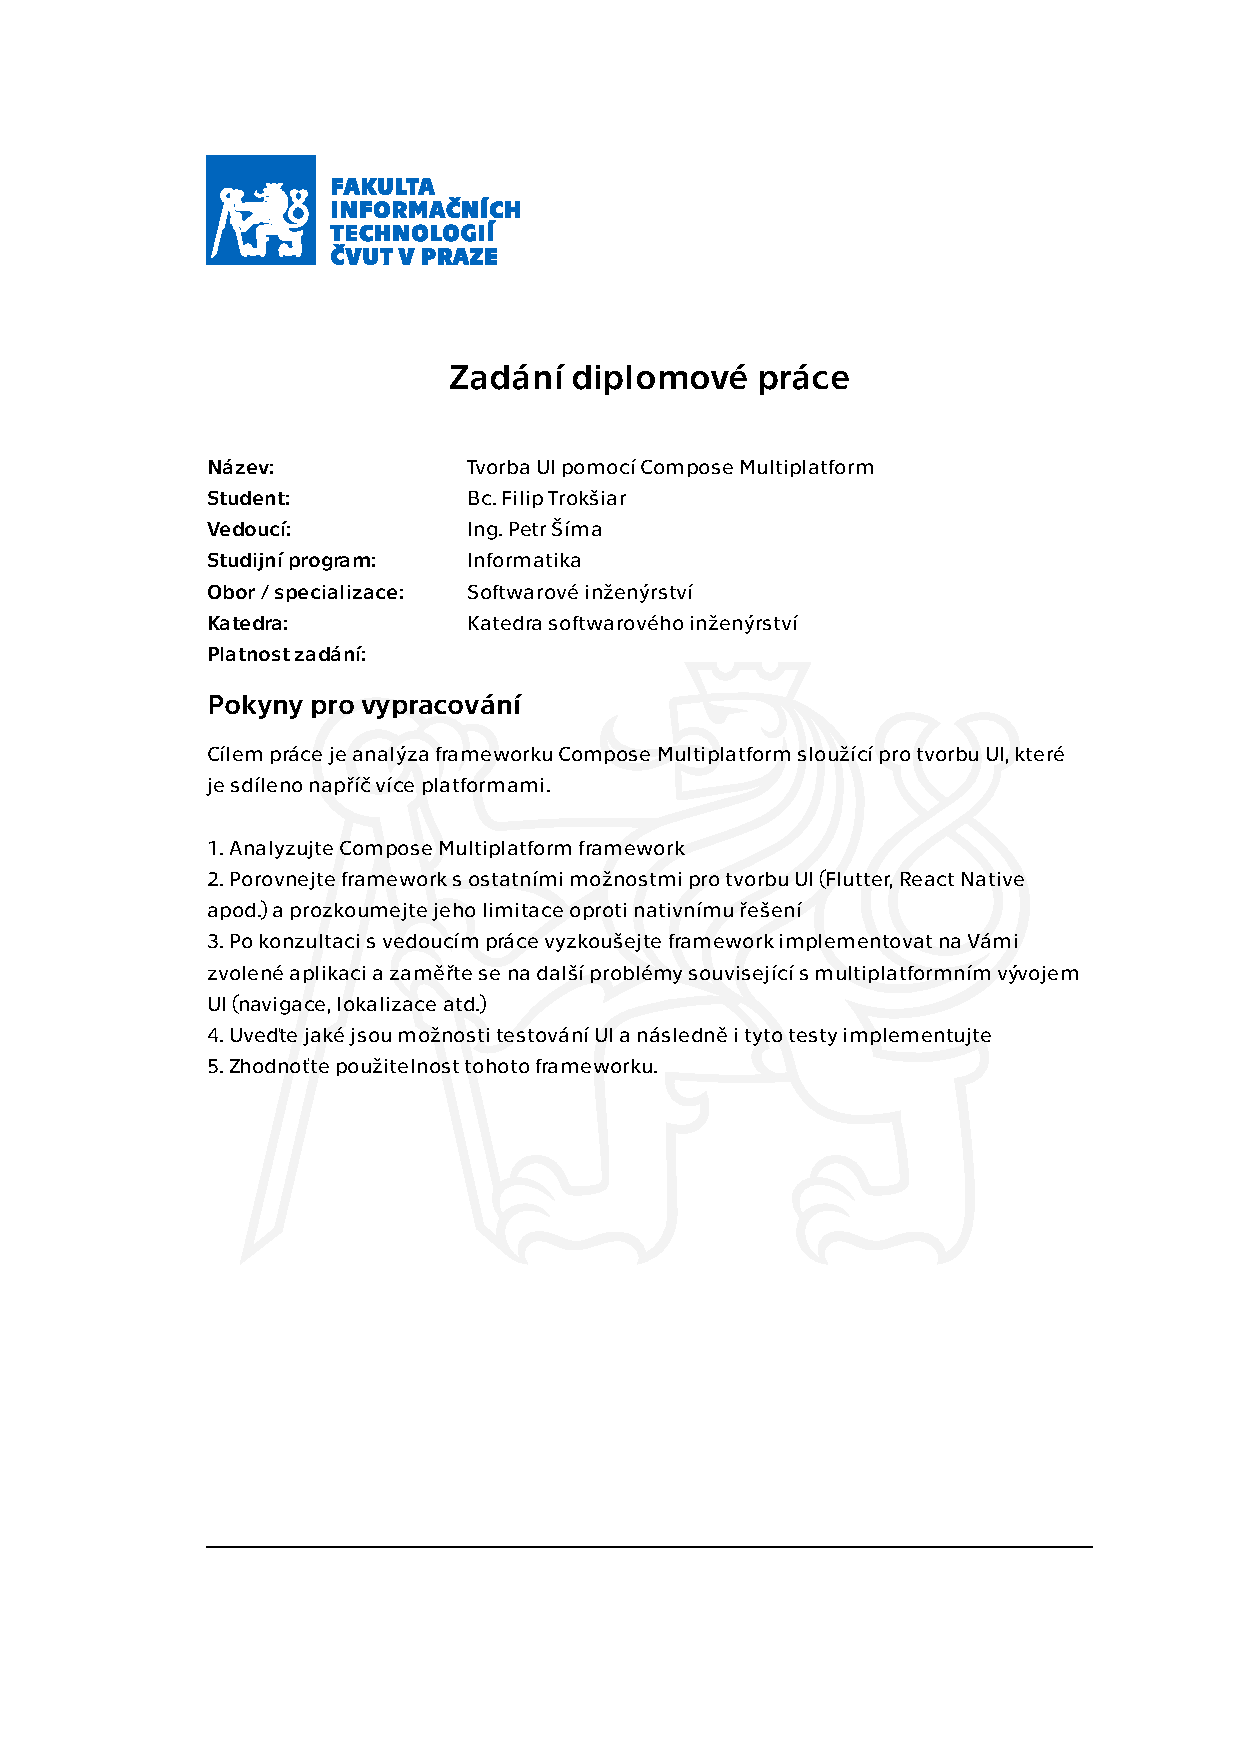
\includepdf[pages={1-}]{troksfil-assignment.pdf} % replace that file with your thesis assignment provided by study office

\thispagestyle{empty}\cleardoublepage\maketitle % do not remove these three commands

\imprintpage % do not remove this command

\tableofcontents % do not remove this command
%%%%%%%%%%%%%%%%%%%%%%
% list of other contents: figures, tables, code listings, algorithms, etc.
% add/remove commands accordingly
%%%%%%%%%%%%%%%%%%%%%%
\listoffigures % list of figures
\begingroup
\let\clearpage\relax
\listoftables % list of tables
\lstlistoflistings % list of source code listings generated by the listings package
% \listoflistings % list of source code listings generated by the minted package
\endgroup
%%%%%%%%%%%%%%%%%%%%%%
% list of other contents END
%%%%%%%%%%%%%%%%%%%%%%

%%%%%%%%%%%%%%%%%%%
% ACKNOWLEDGMENT
% FILL IN / MODIFY
% This is a place to thank people for helping you. It is common to thank your supervisor.
%%%%%%%%%%%%%%%%%%%
\begin{acknowledgmentpage}
	Chtěl bych poděkovat především vedoucímu diplomové práce Ing. Petrovi Šímovi za metodické vedení práce a také své rodině a přítelkyni za podporu během studia.
\end{acknowledgmentpage} 
%%%%%%%%%%%%%%%%%%%
% ACKNOWLEDGMENT END
%%%%%%%%%%%%%%%%%%%


%%%%%%%%%%%%%%%%%%%
% DECLARATION
% FILL IN / MODIFY
%%%%%%%%%%%%%%%%%%%
% INSTRUCTIONS
% ENG: choose one of approved texts of the declaration. DO NOT CREATE YOUR OWN. Find the approved texts at https://courses.fit.cvut.cz/SFE/download/index.html#_documents (document Declaration for FT in English)
% CZE/SLO: Vyberte jedno z fakultou schvalenych prohlaseni. NEVKLADEJTE VLASTNI TEXT. Schvalena prohlaseni najdete zde: https://courses.fit.cvut.cz/SZZ/dokumenty/index.html#_dokumenty (prohlášení do ZP)
% //TODO check if OK
\begin{declarationpage}
    Prohlašuji, že jsem předloženou práci vypracoval samostatně a že jsem uvedl veškeré použité
    informační zdroje v souladu s Metodickým pokynem o dodržování etických principů při přípravě
    vysokoškolských závěrečných prací.
    Beru na vědomí, že se na moji práci vztahují práva a povinnosti vyplývající ze zákona č. 121/2000 Sb.,
    autorského zákona, ve znění pozdějších předpisů, zejména skutečnost, že České vysoké učení
    technické v Praze má právo na uzavření licenční smlouvy o užití této práce jako školního díla podle §
    60 odst. 1 citovaného zákona.
\end{declarationpage}
%%%%%%%%%%%%%%%%%%%
% DECLARATION END
%%%%%%%%%%%%%%%%%%%

\printabstractpage % do not remove this command

%%%%%%%%%%%%%%%%%%%
% SUMMARY
% FILL IN / MODIFY
% OR REMOVE ENTIRELY (upon agreement with your supervisor)
% (appropriate to remove in most theses)
%%%%%%%%%%%%%%%%%%%
% \begin{summarypage}
% \section*{Summary section}
% 
% \lipsum[1][1-8]
% 
% \section*{Summary section}
% 
% \lipsum[2][1-6]
% 
% \section*{Summary section}
% 
% \lipsum[3]
% 
% \section*{Summary section}
% 
% \lipsum[2]
% 
% \section*{Summary section}
% 
% \lipsum[1][1-8] Lorem lorem lorem.
% \end{summarypage}
%%%%%%%%%%%%%%%%%%%
% SUMMARY END
%%%%%%%%%%%%%%%%%%%

%%%%%%%%%%%%%%%%%%%
% ABBREVIATIONS
% FILL IN / MODIFY
% OR REMOVE ENTIRELY
% List the abbreviations in lexicography order.
%%%%%%%%%%%%%%%%%%% //TODO Seznam zkratek
\chapter{Seznam zkratek}
	
\begin{tabular}{rl}
DFA & Deterministic Finite Automaton\\
FA & Finite Automaton\\
LPS & Labelled Prüfer Sequence\\
NFA & Nondeterministic Finite Automaton\\
NPS & Numbered Prüfer Sequence\\
XML & Extensible Markup Language\\
XPath & XML Path Language\\
XSLT & eXtensible Stylesheet Language Transformations\\
W3C & World Wide Web Consortium
\end{tabular}
%%%%%%%%%%%%%%%%%%%
% ABBREVIATIONS END
%%%%%%%%%%%%%%%%%%%

\mainmatter\mainmatterinit % do not remove these two commands

%%%%%%%%%%%%%%%%%%%
% THE THESIS
% MODIFY ANYTHING BELOW THIS LINE
%%%%%%%%%%%%%%%%%%%

% Do not forget to include Introduction
%---------------------------------------------------------------
\chapter{Úvod}
% uncomment the following line to create an unnumbered chapter
%\chapter*{Úvod}\addcontentsline{toc}{chapter}{Introduction}\markboth{Introduction}{Introduction}
%---------------------------------------------------------------
\setcounter{page}{1}

% The following environment can be used as a mini-introduction for a chapter. Use that any way it pleases you (or comment it out). It can contain, for instance, a summary of the chapter. Or, there can be a quotation.
%\begin{chapterabstract}
%	\lipsum[1]
%\end{chapterabstract}

%\section{Motivace}
\section{Cíle práce}
Cílem práce je prozkoumat použitelnost nově 


\section{Stručný přehled obsahu práce}

Obecně něco o multiplatformním vývoji.

%---------------------------------------------------------------
\section{Teoretický úvod}
%---------------------------------------------------------------

\section{Definice multiplatformního vývoje UI}




\section{Význam multiplatformního vývoje a sdíleného UI}

Mezi primární důvody vedoucí firmy a jednotlivce k vývoji multiplatformních aplikací patří především
snížení nákladů na vývoj a následně také na údržbu. Jednodušší dosažení konzistentního vzhledu
na různých platformách nebo například možnost znovu používat komponenty UI na různých platformách.

Mezi další důvody může například patřit možnost rychlejších aktualizací, jelikož nové funkce mohou být 
implementovány jednotně a rychle na všech platformách. 

%Větší dosah jelikož díky sdílení UI lze dosáhnout většího dosahu, protože aplikace mohou být dostupné 

\chapter{Analýza}

\section{Přehled existujících frameworků}

Mezi nejpopulárnější multiplatformní frameworky jednoznačně patří Flutter a React Native. \cite{crossPlatformFrameworksStats}
%---------------------------------------------------------------
\section{Flutter}
%---------------------------------------------------------------
Flutter je open-source softwarový toolkit pro vývoj uživatelských rozhraní (UI). \cite{flutterfaq} Za vývojem stojí společnost Google a je určený k vytváření nativně kompilovaných 
aplikací pro mobilní zařízení, web a desktop z jednoho zdrojového kódu. \cite{flutterfaq}
Byl vydán v roce 2017 a získal značnou popularitu mezi vývojáři díky svému snadnému použití, flexibilitě a schopnostem tvorby UI.

\section*{Klíčové vlastnosti Flutteru}

\begin{itemize}
    \item \textbf{Architektura založená na widgetech:} Flutter využívá reaktivní a deklarativní architekturu založenou na widgetech. Widgety jsou základními stavebními bloky Flutter aplikací, představující vše od strukturálních prvků po stylistické komponenty.

    \item \textbf{Hot Reload:} Jednou z výrazných funkcí Flutteru je možnost "Hot Reload". Vývojáři mohou provádět změny v kódu a okamžitě vidět výsledky bez restartování aplikace. To zrychluje vývojový proces a zvyšuje produktivitu.

    \item \textbf{Jeden zdrojový kód pro více platforem:} S Flutterem mohou vývojáři psát jeden zdrojový kód pro obě platformy Android a iOS, což snižuje dobu vývoje a úsilí vynakládané na údržbu. Flutter také rozšířil svou podporu pro cílení webových a desktopových aplikací, umožňující širší dosah s minimálními změnami kódu.

    \item \textbf{Rozsáhlá sada widgetů:} Flutter poskytuje komplexní sadu přizpůsobitelných widgetů, které usnadňují vytváření složitých a vizuálně atraktivních uživatelských rozhraní. Tyto widgety zahrnují vše od základních tlačítek a textových polí až po pokročilé komponenty jako jsou grafy a animace.

    \item \textbf{Programovací jazyk Dart:} Aplikace vytvořené ve Flutteru jsou psány v jazyce Dart, moderním objektově orientovaném programovacím jazyce vyvinutém společností Google. Dart je navržen pro optimální výkon a produktivitu, což ho činí vhodným pro mobilní a webový vývoj.

    %\item \textbf{Výkon:} Flutter se kompiluje do nativního ARM kódu, což vede k vysokému výkonu aplikací. Vrstvená architektura frameworku umožňuje detailní kontrolu nad vzhledem a chováním aplikací.

\end{itemize}

\section*{Architektura Flutteru} 

Během vývoje běží Flutter aplikace na virtuálním počítači, který nabízí takzvaný stateful Hot Reload umožňující zobrazit provedené změny
v kódu bez nutnosti úplné rekompilace aplikace. Teprve pro vydání jsou Flutter aplikace kompilovány přímo do strojového kódu, 
ať už jde o instrukce Intel x64 nebo ARM, případně do JavaScriptu pokud jsou cíleny na web. \cite{flutterArchOverview}

\medskip

Jak je vidět na obrázku \ref{fig:flutter_architectural_layers}, tak architektura Flutteru je rozdělena do tří hlavních vrstev.
Embedder je vrstva, která umožnuje integrovat Flutter do konkrétních platforem jako je Android, iOS, desktop nebo web. 
Každý embedder obsahuje platformě specifický kód, který je potřebný pro spuštění Flutteru na dané platformě.
Engine je vrstva starající se o vykreslování grafiky, kdykoli kdy je potřeba vykreslit nový snímek. \cite*{flutterArchOverview} 
Framework je vrstva, která je používána vývojáři k vytváření uživatelských rozhraní a definování chování aplikace. 
Obsahuje hotové widgety, funkce pro manipulaci s UI a další nástroje pro vývojáře. \cite{flutterArchOverview} 


\begin{figure}[H]
  \centering
  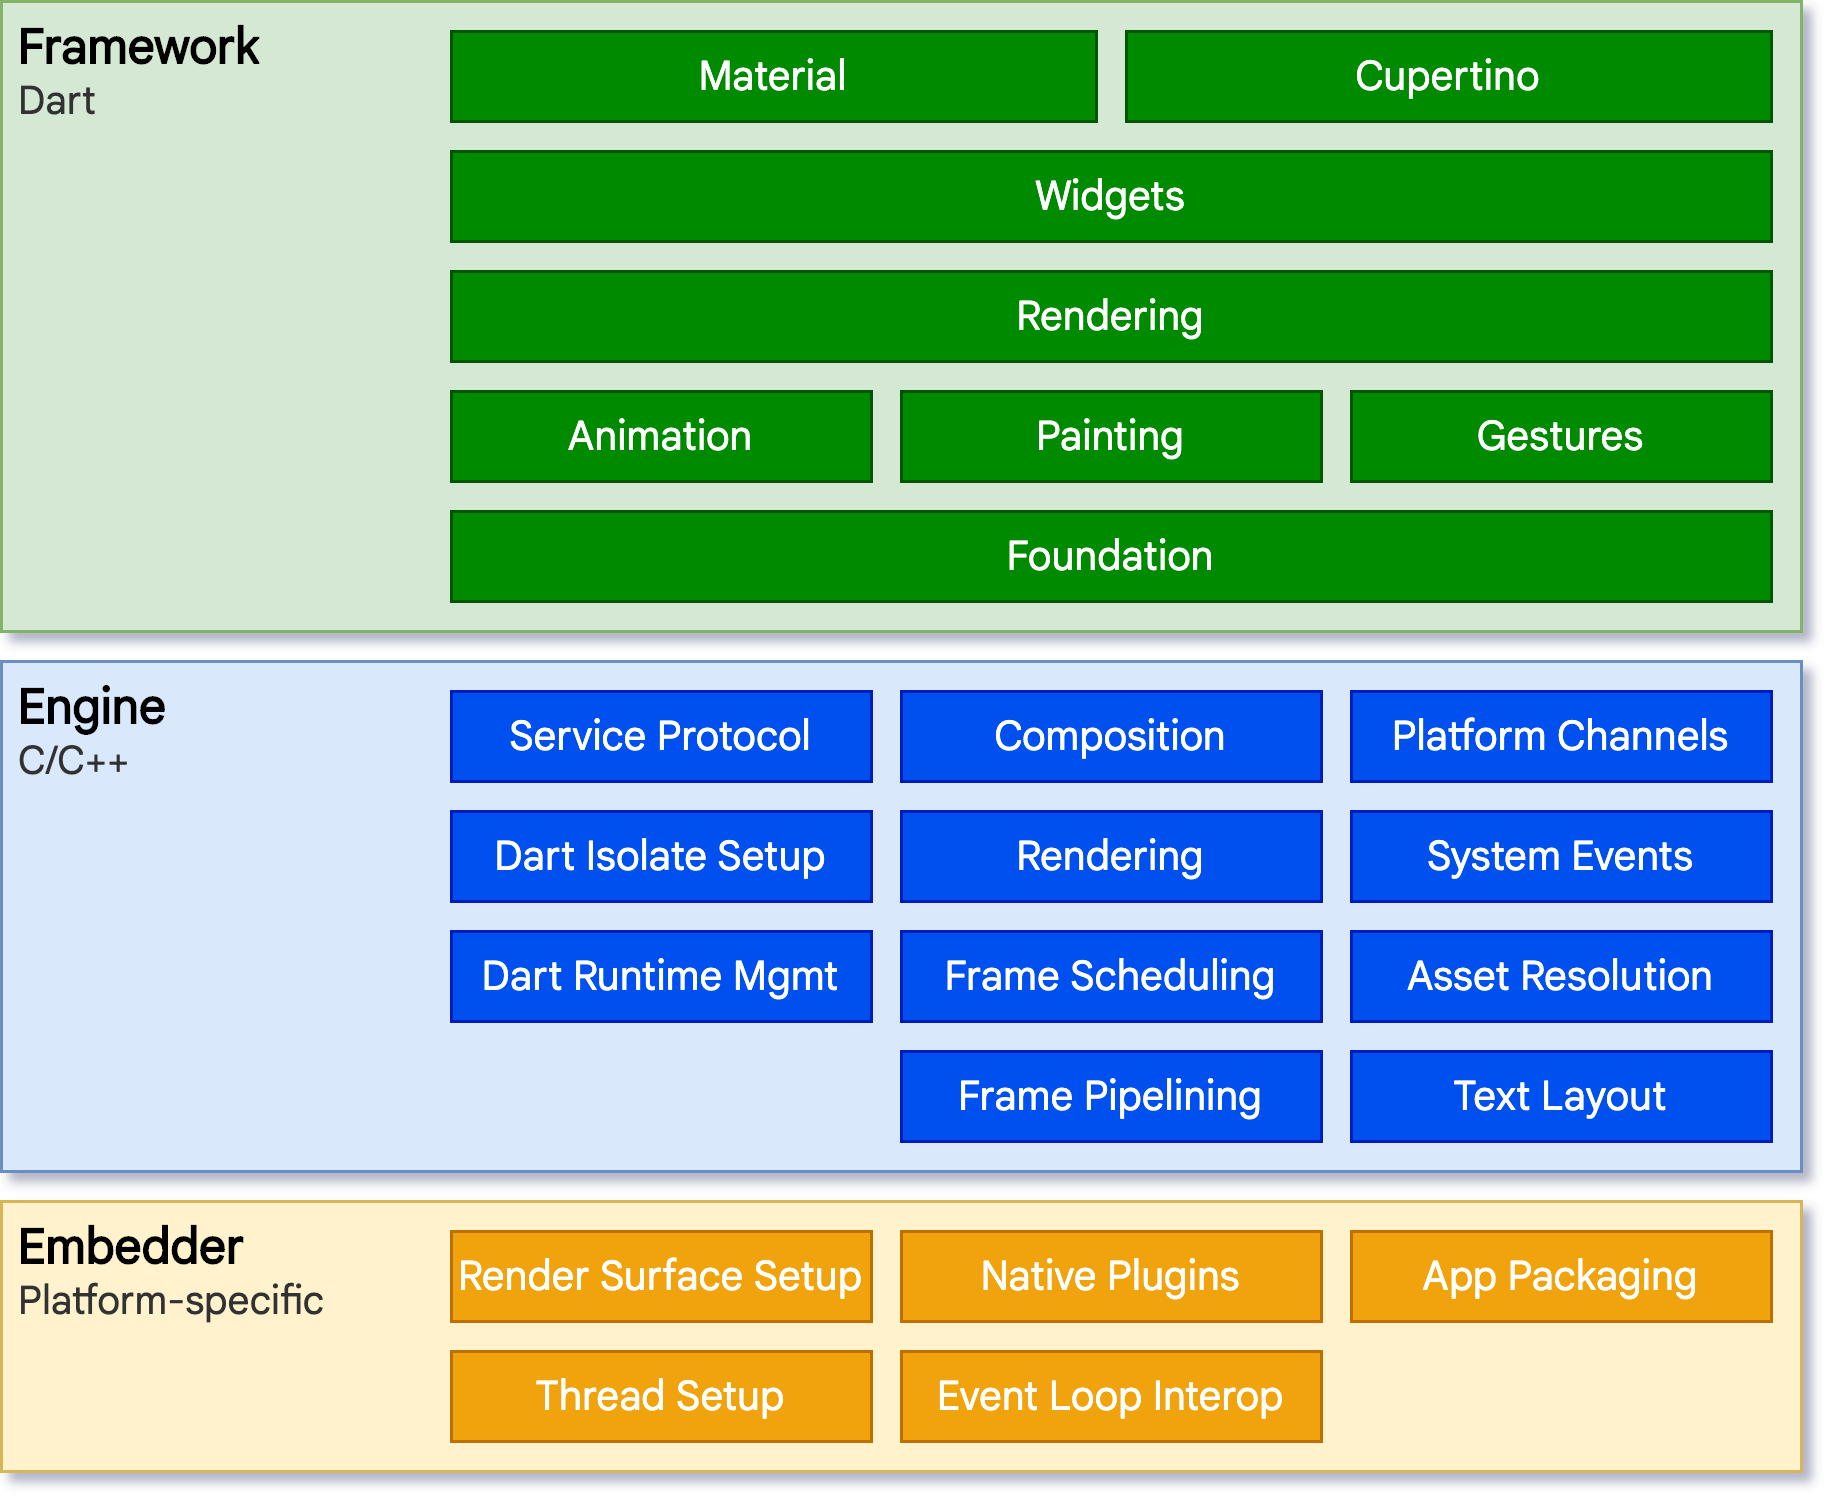
\includegraphics[width=0.85\textwidth]{flutter_architectural_layers.png}
  \caption{Flutter architectural layers}
  \label{fig:flutter_architectural_layers}
\end{figure}

Mezi hierarchicky poslední a neméně důležitou častí tohoto frameworku jsou platformově specifické knihovny Material and Cupertino. Tyto knihovny
jsou následně využívány widgety k implementaci konkrétního design systému. Díky tomu je možné uživateli navodit nativní pocit z dané aplikace.

\medskip

Z pohledu UI je důležitým prvkem právě Flutter framework, který zároveň definuje jak spolu jednotlivé widgety interagují.

Widget je ve Flutteru základní stavební blok pro tvorbu uživatelského rozhraní. V následující ukázce kódu je pro příklad použito několik 
základních widgetů jako je \emph{Image} nebo \emph{Text} a taktéž layout widgety zvané \emph{Container} a \emph{Row} pro organizaci a 
rozložení vnořených widgetů na obrazovce.

\begin{lstlisting}
  Container(
  color: Colors.blue,
  child: Row(
    children: [
      Image.network('https://www.example.com/1.png'),
      const Text('A'),
    ],
  ),
);
\end{lstlisting}

Když Flutter potřebuje vykreslit tento blok, zavolá metodu \emph{build()} a ta vrátí podstrom widgetů, které následně vykreslí uživatelské 
rozhraní na základě aktuálního stavu aplikace. \cite*{flutterArchOverview}

Během fáze sestavování překládá Flutter widgety vyjádřené v kódu do odpovídajícího stromu elementů, přičemž každý widget má jeden element a 
každý prvek představuje určitou instanci widgetu v daném umístění stromové hierarchie. \cite*{flutterArchOverview}


\begin{figure}[H]
  \centering
  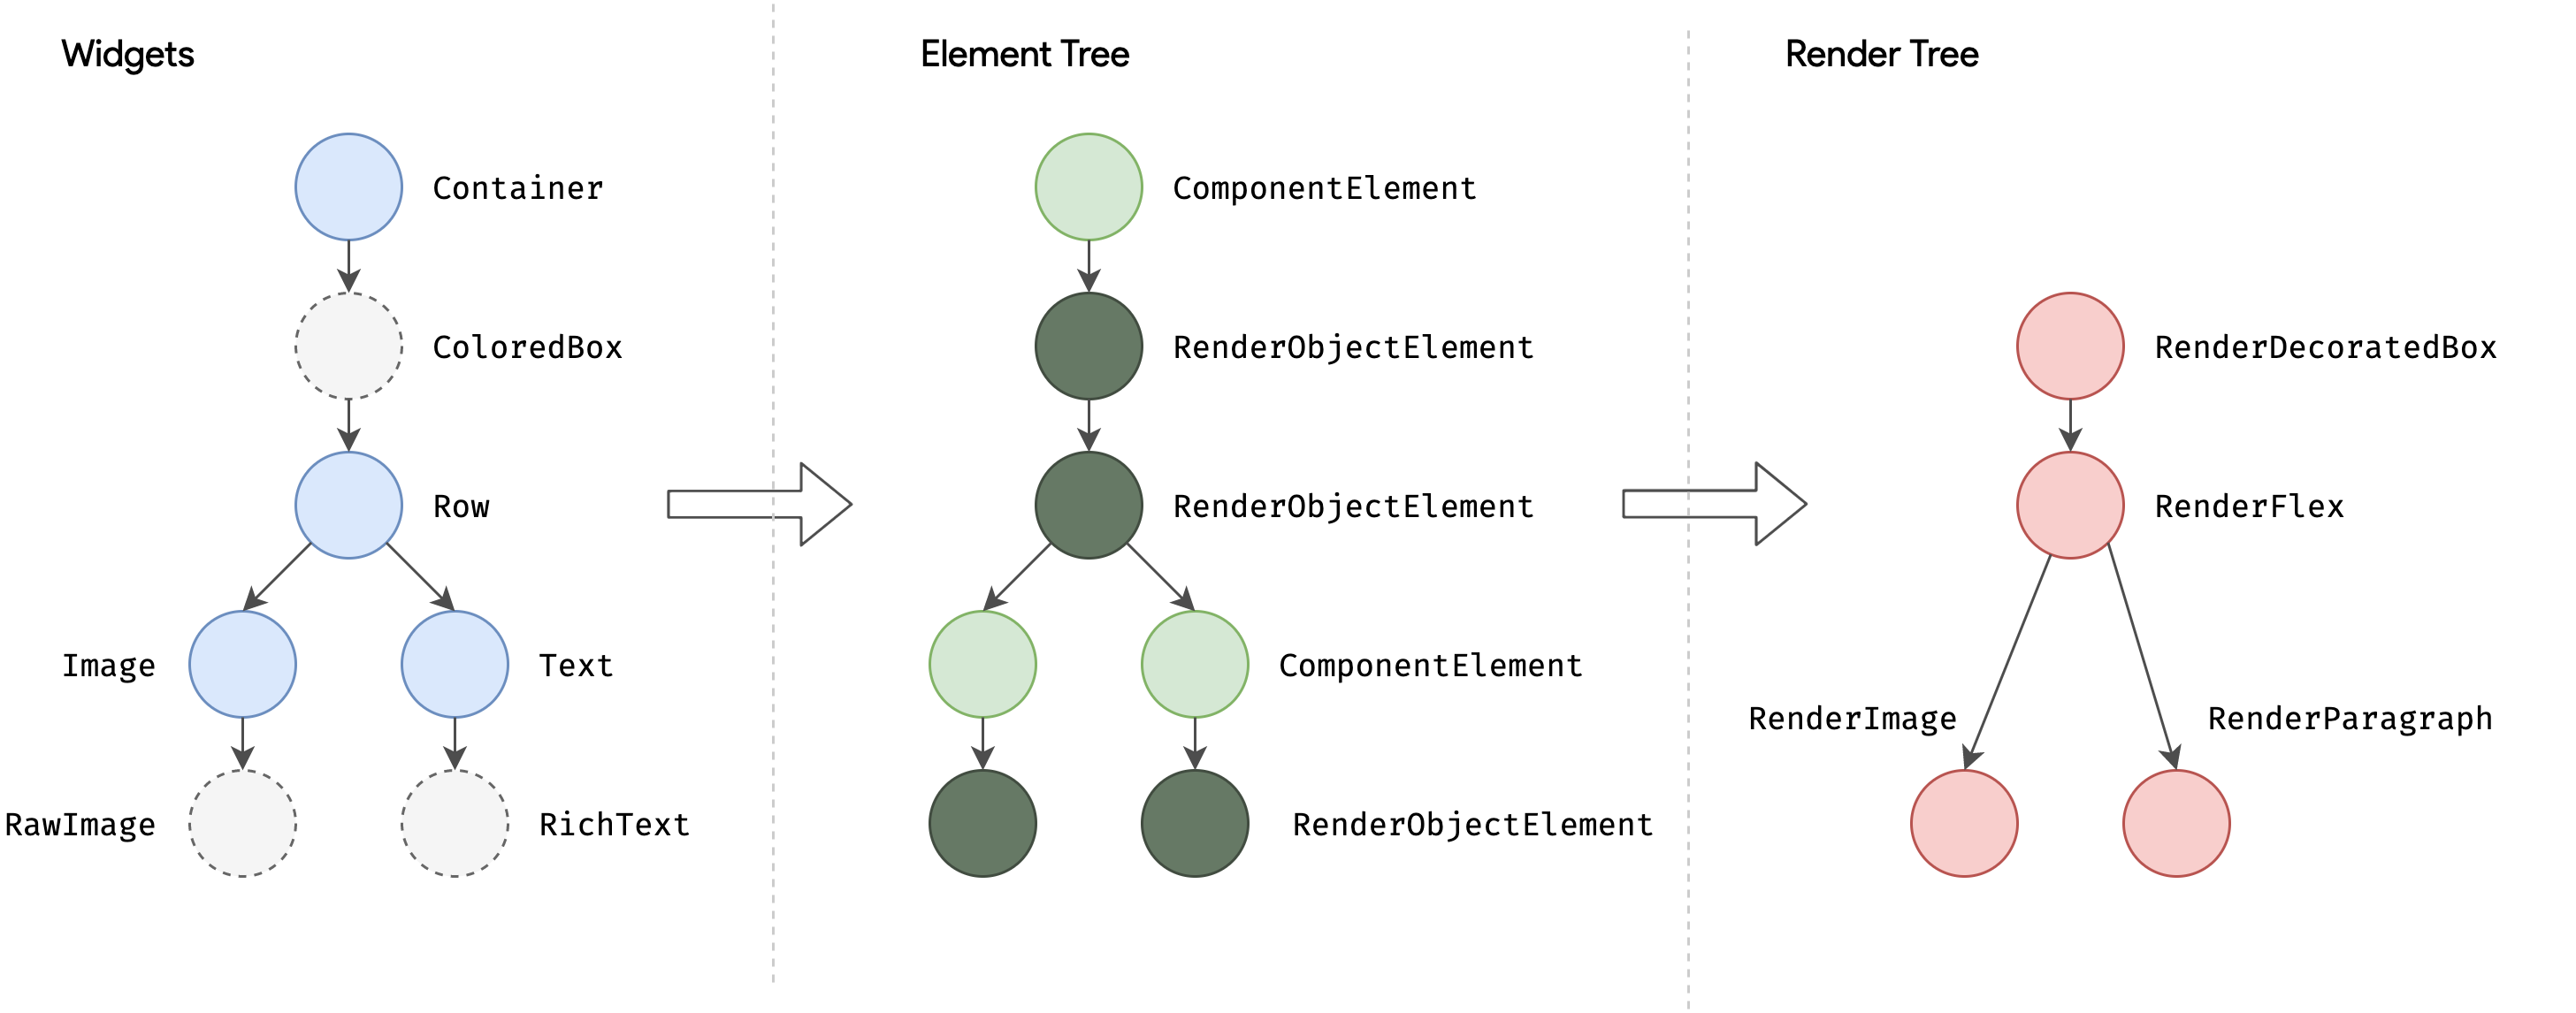
\includegraphics[width=1\textwidth]{flutter_trees.png}
  \caption{Flutter build proces}
  \label{fig:flutter_trees}
\end{figure}





%---------------------------------------------------------------
\section{React Native}
%---------------------------------------------------------------

React Native je open-source framework pro vývoj mobilních aplikací, vyvinutý společností Facebook. Jeho hlavním cílem je umožnit vývojářům vytvářet nativní mobilní aplikace pro platformy Android a iOS z jednoho společného kódu napsaného v jazyce JavaScript nebo TypeScript.

\section*{Klíčové vlastnosti React Native}

\begin{itemize}
    \item \textbf{Komponentní architektura:} React Native využívá komponentní architekturu, která umožňuje vytvářet znovupoužitelné a modulární komponenty. 

    \item \textbf{Hot Reload:} Podobně jako u Flutteru, React Native nabízí funkci "Hot Reload," což umožňuje vývojářům okamžitě vidět výsledky svých změn v kódu bez nutnosti restartování aplikace.

    \item \textbf{Jednotný kód pro Android a iOS:} React Native umožňuje vývojářům sdílet většinu kódu mezi Androidem a iOS, což snižuje náklady na vývoj a usnadňuje správu projektu.

    \item \textbf{JavaScript/TypeScript:} Aplikační logika v React Native se píše v jazyce JavaScript nebo TypeScript, což usnadňuje integraci s existujícími webovými technologiemi.

    \item \textbf{Rozsáhlá komunita:} React Native má rozsáhlou komunitu vývojářů, což vede k bohatému ekosystému třetích stran, včetně mnoha dostupných knihoven a modulů.

    \item \textbf{Expo framework:} Pro ještě snazší start vývoje poskytuje React Native Expo framework, který zjednodušuje proces vývoje a umožňuje rychlé prototypování.

\end{itemize}

\section*{Flutter vs React Native vs Compose Multiplatform}




\section{Compose Multiplatform Framework}

Compose Multiplatform je framework sloužící k tvorbě uživatelských rozhraní použitelných na vícero platformách za 
jehož vývojem stojí společnost JetBrains. \cite{composeMultiplatform} Je založen na toolkitu zvaném Jetpack Compose, který je aktuálně 
doporučovaný k tvorbě nativních uživatelských rozhraních na platformě Android. \cite{jetpack}

\medskip

Mezi klíčové vlastnosti tohoto frameworku patří:

\begin{itemize}
    \item \textbf{Deklarativní syntaxe:} Používá deklarativní syntaxi pro popis uživatelského rozhraní.
    \item \textbf{Jednotný kód pro různé platformy:} Možnost sdílet kód pro Android, iOS, Desktop i Web.
    \item \textbf{Programovací jazyk Kotlin:} Frontendová i backendová část aplikace jsou psány v jazyce Kotlin pro bezproblémovou integraci se serverovou částí.
    \item \textbf{Podpora od JetBrains:} Poskytuje stabilní podporu od vývojářského týmu JetBrains.
\end{itemize}

\subsection{Kotlin Multiplatform}


%https://blog.jetbrains.com/kotlin/2023/11/kotlin-multiplatform-stable/#use-the-power-of-the-growing-kotlin-multiplatform-ecosystem

Kotlin Multiplatform je často základním kamenem pro tvorbu multiplatformních aplikací založených na Compose Multiplatform. Jelikož se jedná o SDK, 
tak umožňuje vývojářům implementovat multiplatformní funkcionality postupně, bez nutnosti implementovat v Kotlinu celé vrstvy aplikací. 

Od listopadu 2023 má svoji stabilní verzi, která je stoprocentně připravena na produkční nasazení. \cite{KMPstable}

\begin{figure}[H]
  \centering
  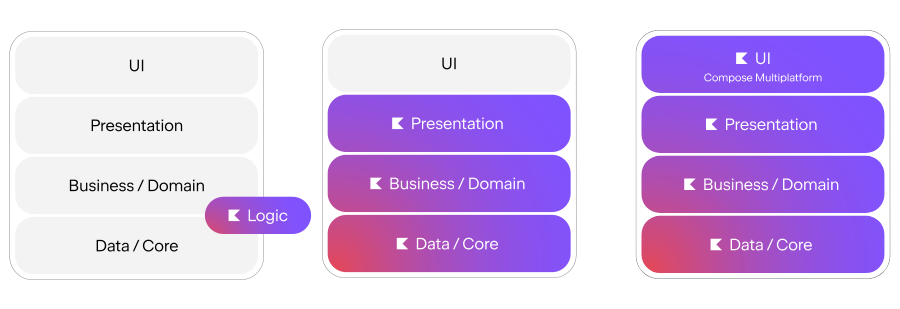
\includegraphics[width=1\textwidth]{KMP_vrstvy.png}
  \caption{Možnosti implementace KMP}
  \label{fig:KMP_vrstvy}
\end{figure}



\begin{figure}[H]
  \centering
  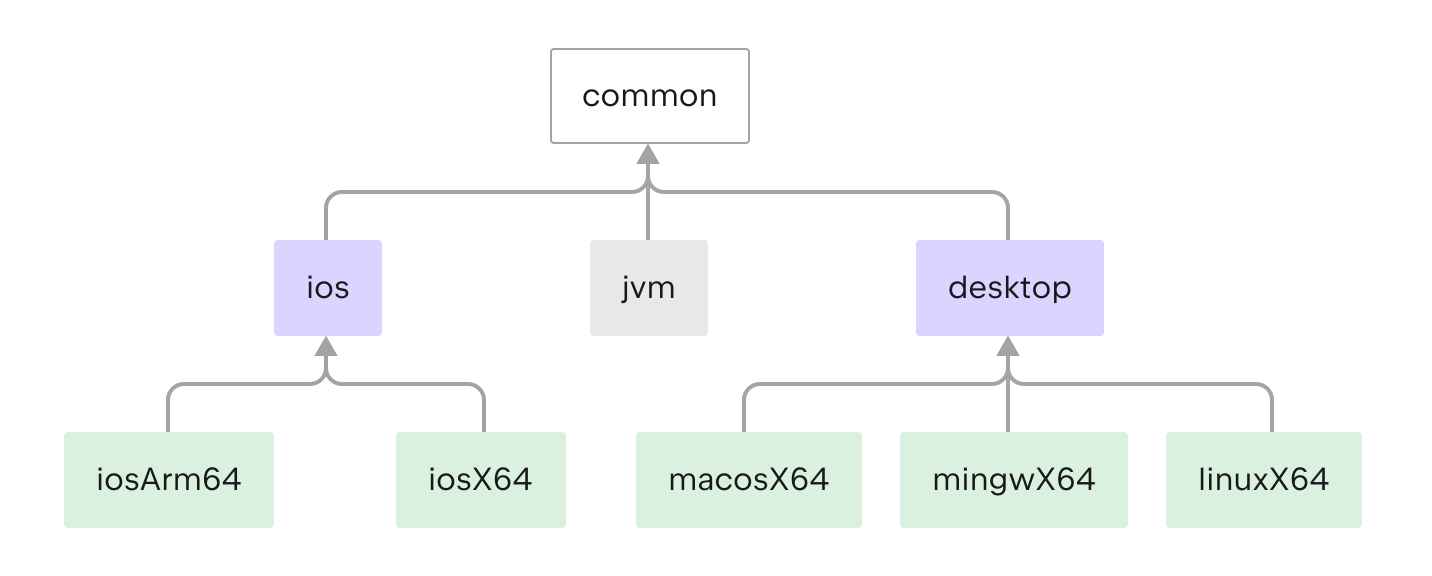
\includegraphics[width=1\textwidth]{kotlin-multiplatform-hierarchical-structure.png}
  \caption{Hierarchická struktura KMP}
  \label{fig:KMP_struktura}
\end{figure}

\subsubsection{Aktuální použití KMP v praxi}


\emph{"Od této doby jsme vyvinuli a v produkci provozujeme několik mobilních aplikací. Ze zkušenosti vidíme, že při jejich vývoji dokážeme sdílet cca 60–70 \% kódu na platformu. V případě vývoje na dvě platformy to znamená, že v součtu dokážeme ušetřit minimálně třetinu nákladů na vývoj, plus s tím související další náklady na věci typu testování (v tomto případě snížení až na polovinu)."}

\begin{figure}[H]
  \centering
  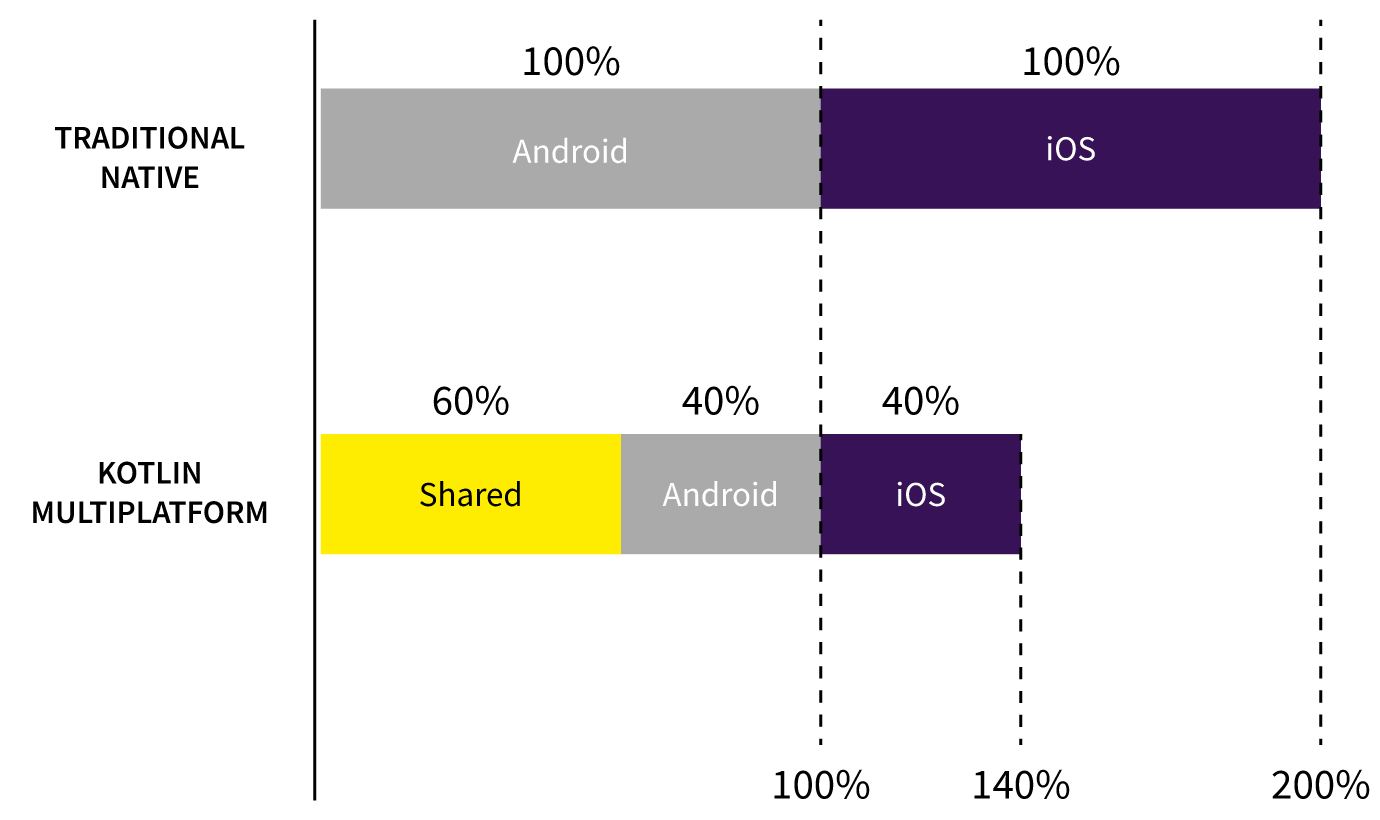
\includegraphics[width=.7\textwidth]{chart-KMP-vs-native.png}
  \caption{Množství kódu KMP vs native}
  \label{fig:KMP_vs_native}
\end{figure}

\section{Omezení výkonu}


\section{Ukázková aplikace}

Aplikace obsahovala jednu obrazovku, načetla obrázky z veřejného API a zobrazila je v horizontálním seznamu. 
Na každý obrázek šlo kliknout a zobrazit jej přiblížený pod seznamem. 
Pro testování byly použity nativní toolkity Jetpack Compose a SwiftUI, dále Compose Multiplatform a framework Flutter.  


Na obrázku \ref*{fig:chart_app_sizes} je vidět ja 

\begin{figure}[H]
  \centering
  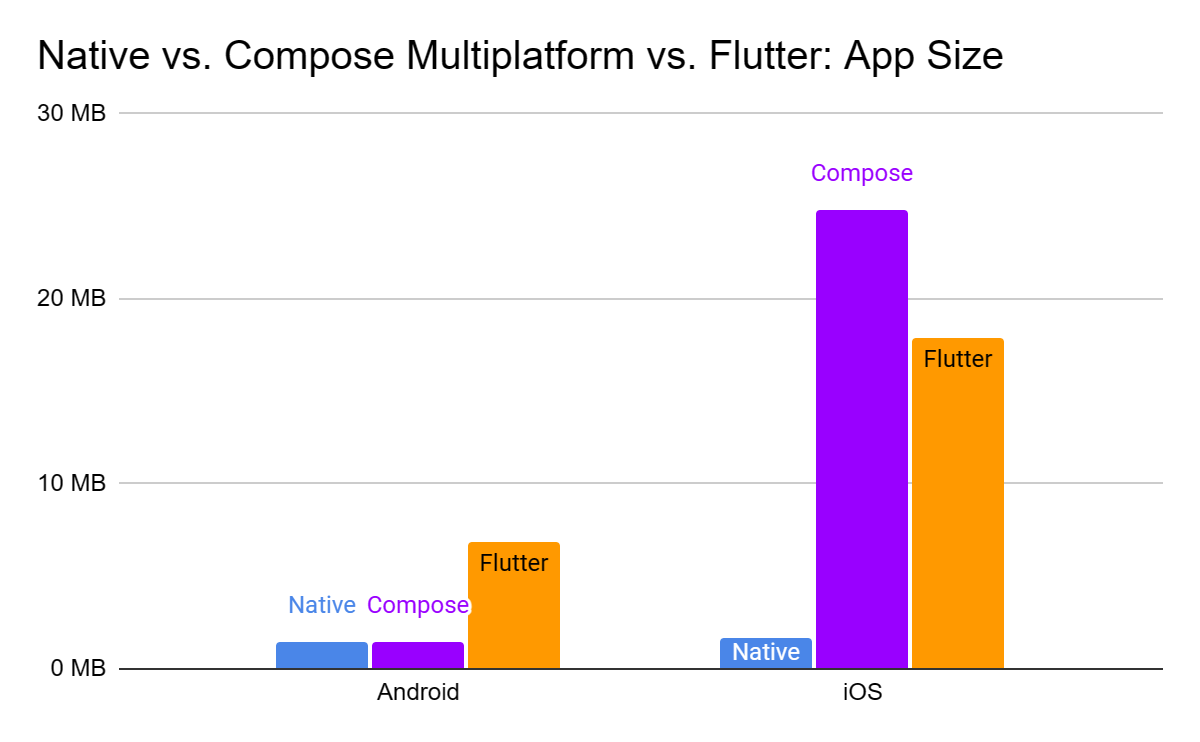
\includegraphics[width=.7\textwidth]{chart_app_sizes.png}
  \caption{APK/IPA size in megabytes}
  \label{fig:chart_app_sizes}
\end{figure}

\begin{figure}[H]
  \centering
  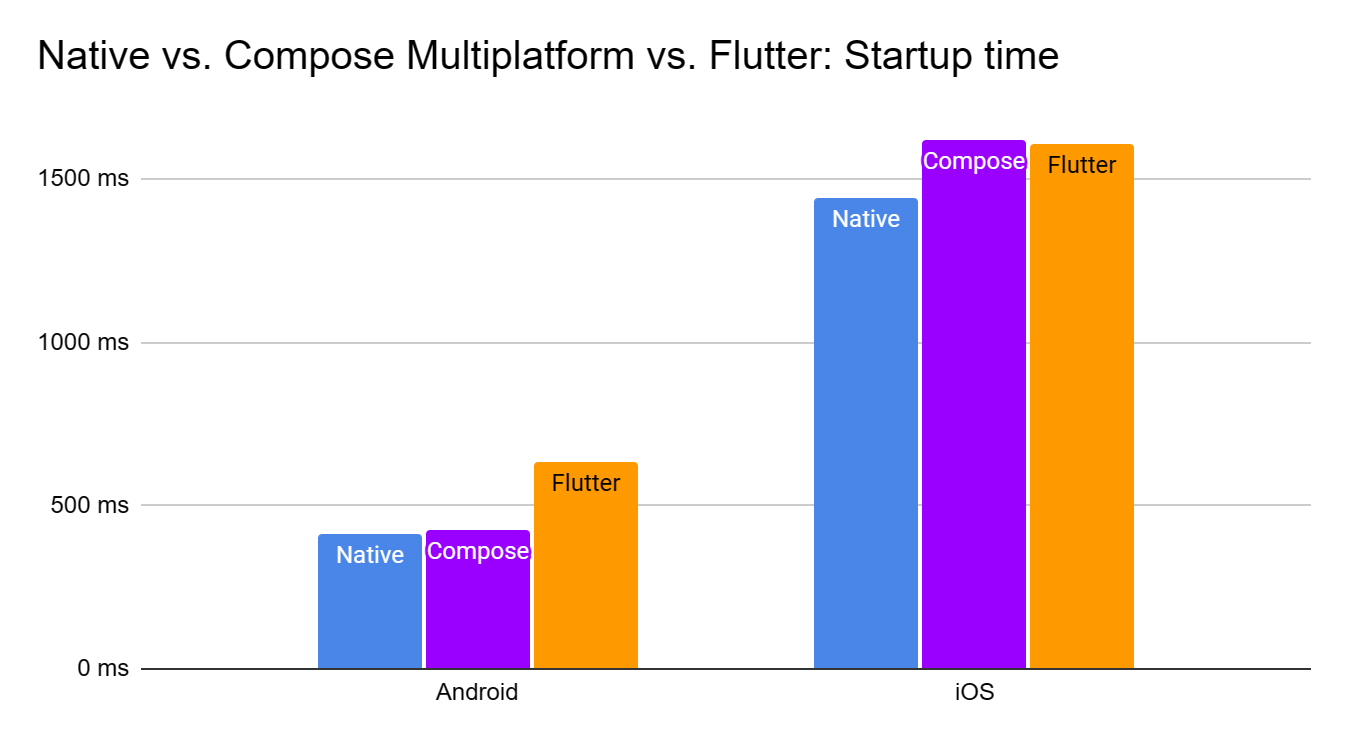
\includegraphics[width=.7\textwidth]{chart_startup_times.png}
  \caption{App startup time on a Pixel 4a and iPhone 12 Mini in milliseconds}
  \label{fig:chart_startup_times}
\end{figure}

\section{Náročnost implementace}
\section{Omezení možností UI designu}

\begin{figure}[H]
    \centering
    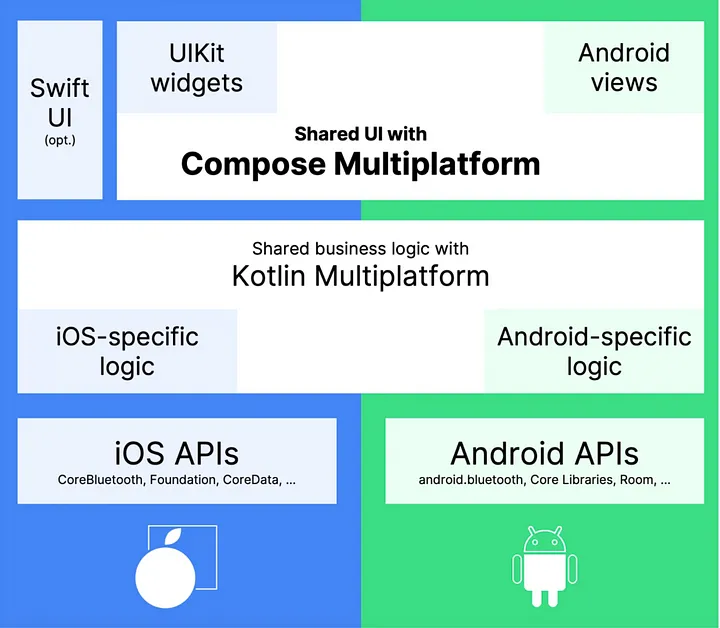
\includegraphics[width=.7\textwidth]{composeIOS.png}
    \caption{Compose Multiplatform iOS}
    \label{fig:composeIOS}
\end{figure}

\chapter{Návrh}



\section{Výběr aplikace pro implementaci}
Základním požadavkem bylo vybrat takovou aplikaci, ve které by bylo možné použít velké množství různých komponent, které by bylo možné použít napříč různými platformami.
Mezi další požadavky patřilo například využití  

Z těchto důvodů byla k iplemenci vybrána aplikace sloužící pro občany měst či obcí, která by sloužila jako p



\section{Návrh UI}

\begin{figure}[H]
    \minipage{0.4\textwidth}
      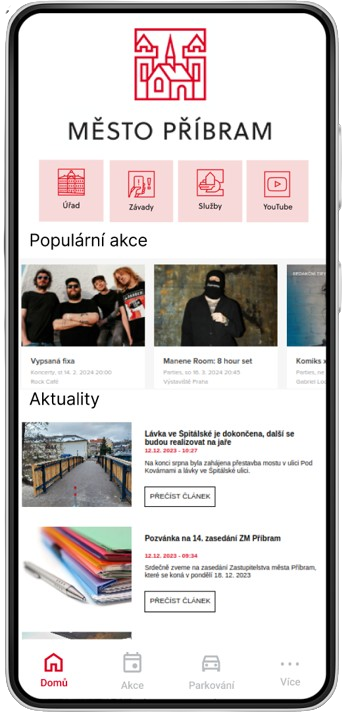
\includegraphics[width=\linewidth]{screen1.png}
      \caption{Screen 1}\label{fig:screen1}
    \endminipage\hfill
    \minipage{0.4\textwidth}
      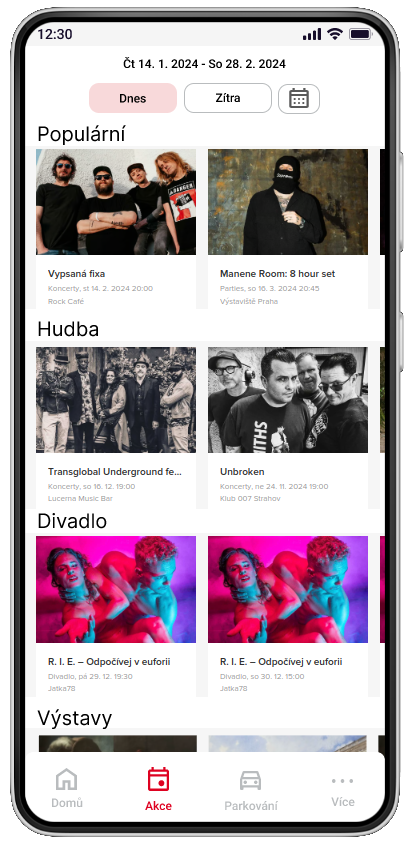
\includegraphics[width=\linewidth]{screen2.png}
      \caption{Screen 2}\label{fig:screen2}
    \endminipage\hfill
\end{figure}

\begin{figure}[H]
    \minipage{0.4\textwidth}
    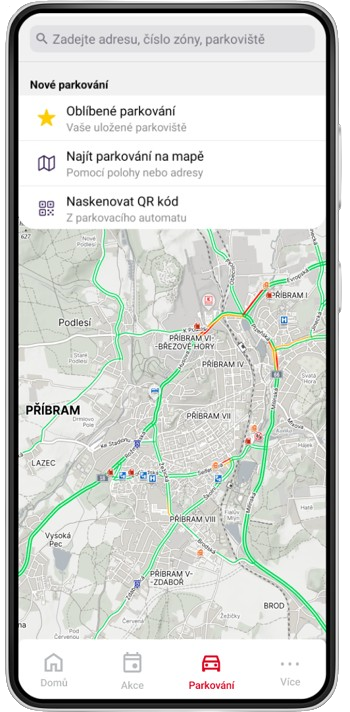
\includegraphics[width=\linewidth]{screen3.png}
    \caption{Screen 3}\label{fig:screen3}
  \endminipage\hfill
  \minipage{0.4\textwidth}
    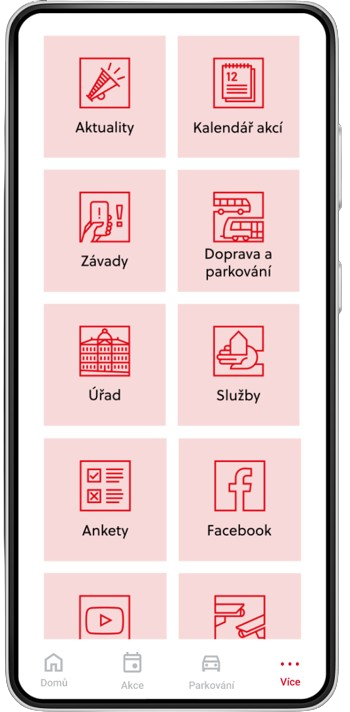
\includegraphics[width=\linewidth]{screen4.png}
    \caption{Screen 4}\label{fig:screen4}
  \endminipage\hfill
\end{figure}

\section{Návrh architektury}

\begin{figure}[H]
  \centering
  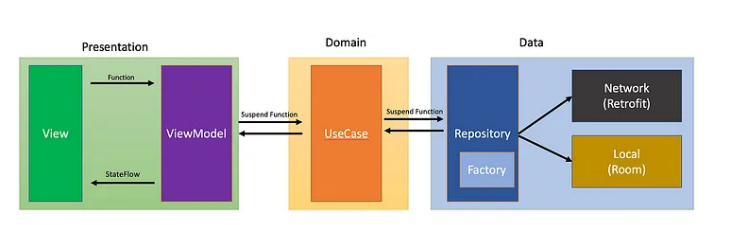
\includegraphics[width=1\textwidth]{mvvm.png}
  \caption{MVVM with Clean Architecture}
  \label{fig:mvvm}
\end{figure}

\dirtree{%
        .1 src \DTcomment{}.
        .2 androidMain \DTcomment{}.
        .2 commonMain \DTcomment{je pro kód sdílený mezi všemi platformami}.
        .3 kotlin \DTcomment{}.
        .4 data\DTcomment{datová vrstva}.
		.5 model\DTcomment{}.
		.5 repository.
		.4 ui\DTcomment{prezentační vrstva}.
		.5 composables\DTcomment{}.
		.5 screens\DTcomment{}.
		.6 HomeScreen\DTcomment{}.
        .3 resourses \DTcomment{}.
        .2 desktop Main \DTcomment{}.
	}




\chapter{Implementace}

\section{Řešení problémů spojených s multiplatformním vývojem}
\section{Navigace a lokalizace v implementaci}

\chapter{Testování}

\section{Možnosti testování UI v Compose Multiplatform}
\section{Implementace testů}
\section{Zhodnocení výsledků testování}

\section{Zhodnocení použitelnosti}

\chapter{Závěr}

\section{Evaluace vlastností Compose Multiplatform ve srovnání s cíli práce}
\section{Zkušenosti z implementace na reálné aplikaci}
\section{Závěr o použitelnosti frameworku}

\section{Shrnutí dosažených výsledků}
\section{Zhodnocení splnění cílů práce}
\section{Návrhy pro budoucí vývoj a výzkum}


 % include `text.tex' from `text/' subdirectory

\appendix\appendixinit % do not remove these two commands

\chapter{Snímky obrazovky}

\begin{figure}[H]
    \minipage{0.4\textwidth}
    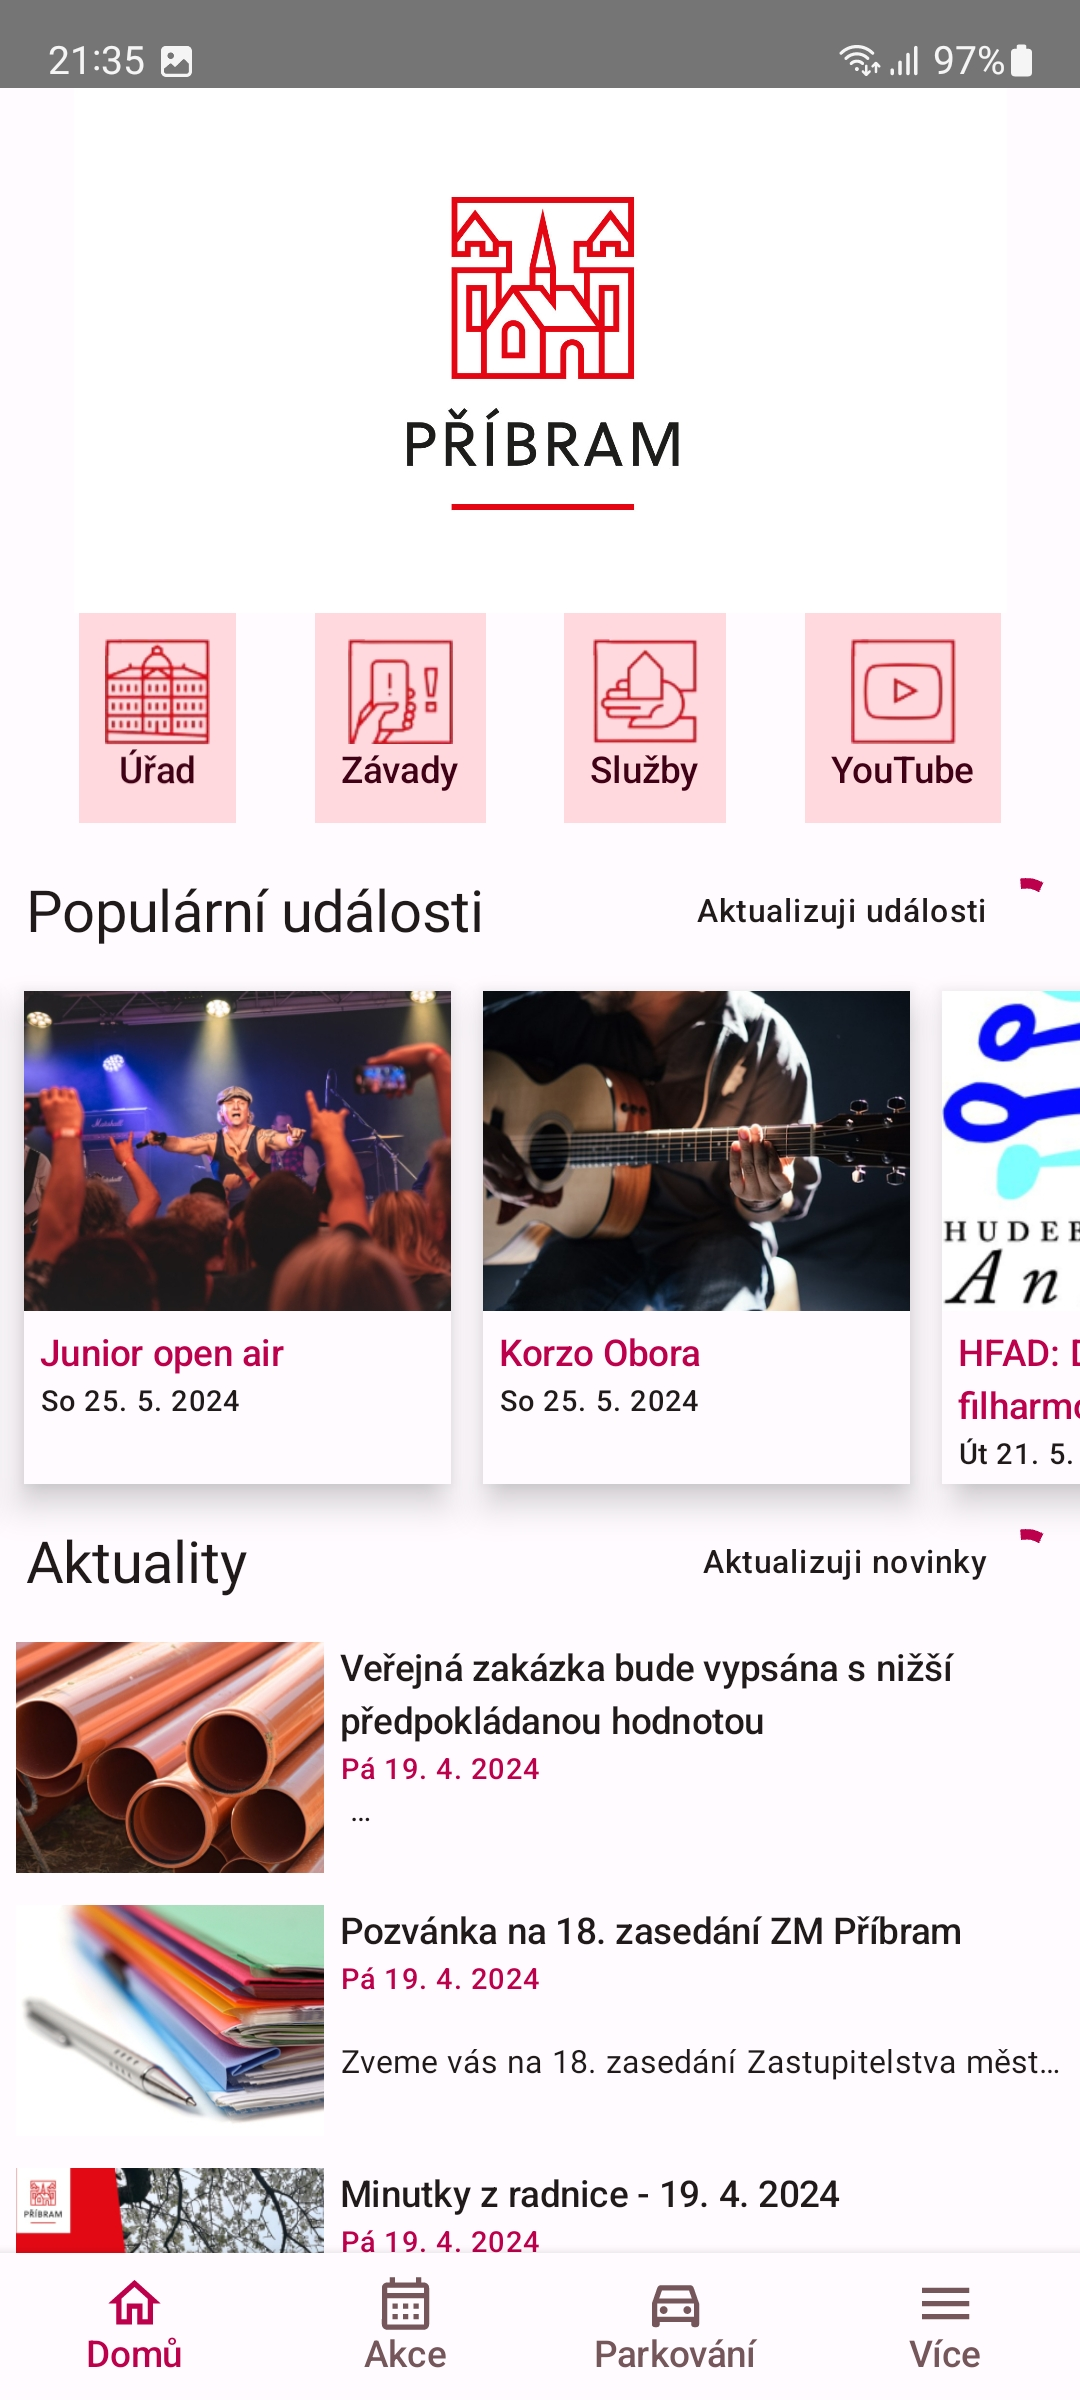
\includegraphics[width=\linewidth]{screens/1.jpg}
    \caption{Domácí obrazovka}
  \endminipage\hfill
  \minipage{0.4\textwidth}
    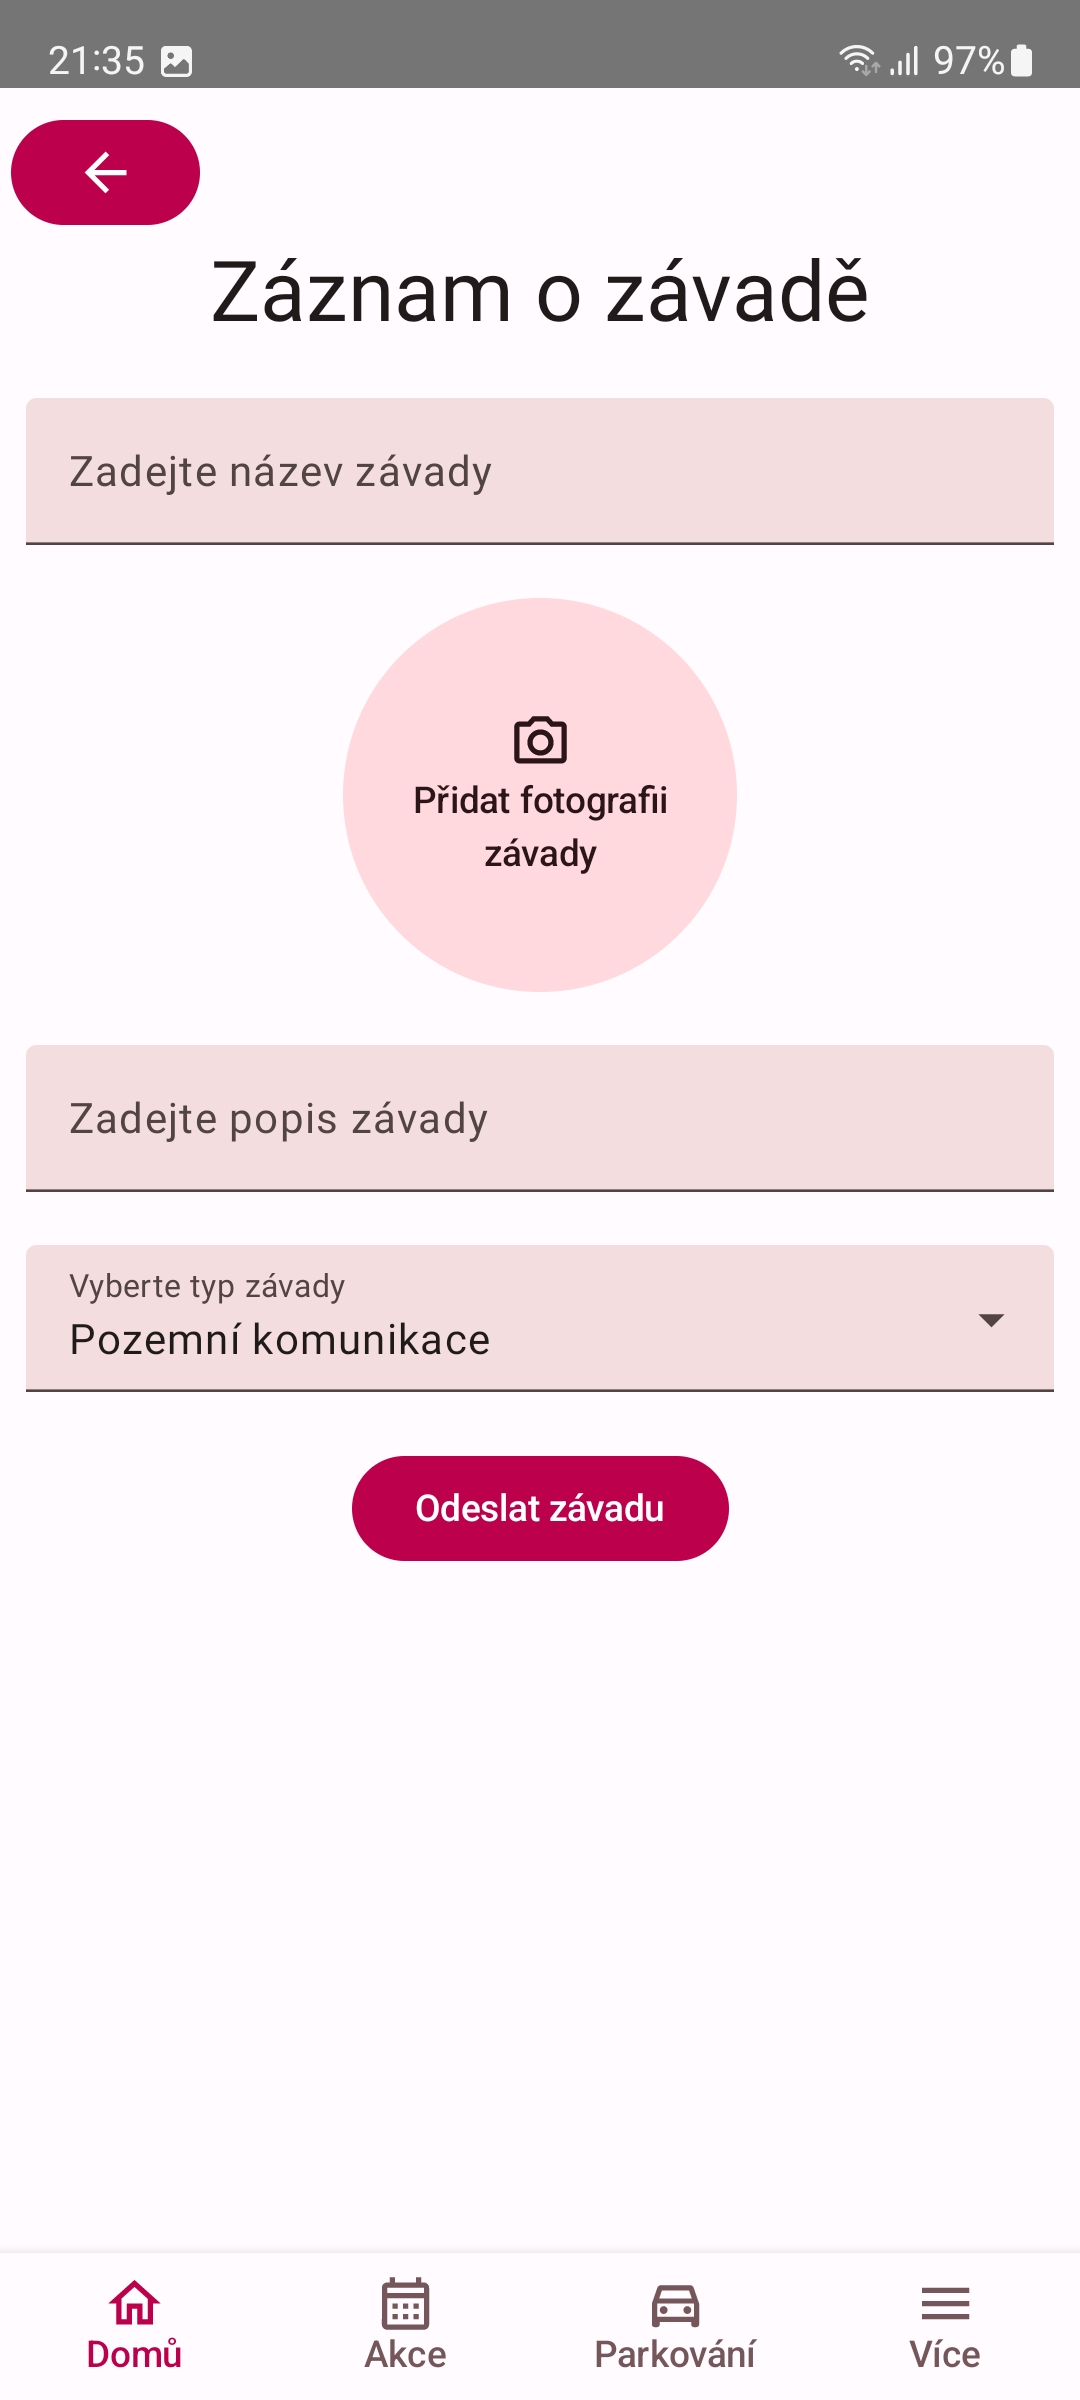
\includegraphics[width=\linewidth]{screens/1b.jpg}
    \caption{Domácí obrazovka}
  \endminipage\hfill
\end{figure}

\begin{figure}[H]
    \minipage{0.4\textwidth}
    
\includegraphics[width=\linewidth]{screens/1e.jpg}
    \caption{Domácí obrazovka}
  \endminipage\hfill
  \minipage{0.4\textwidth}
    
\includegraphics[width=\linewidth]{screens/1e.jpg}
    \caption{Domácí obrazovka}
  \endminipage\hfill
\end{figure}

\begin{figure}[H]
    \minipage{0.4\textwidth}
    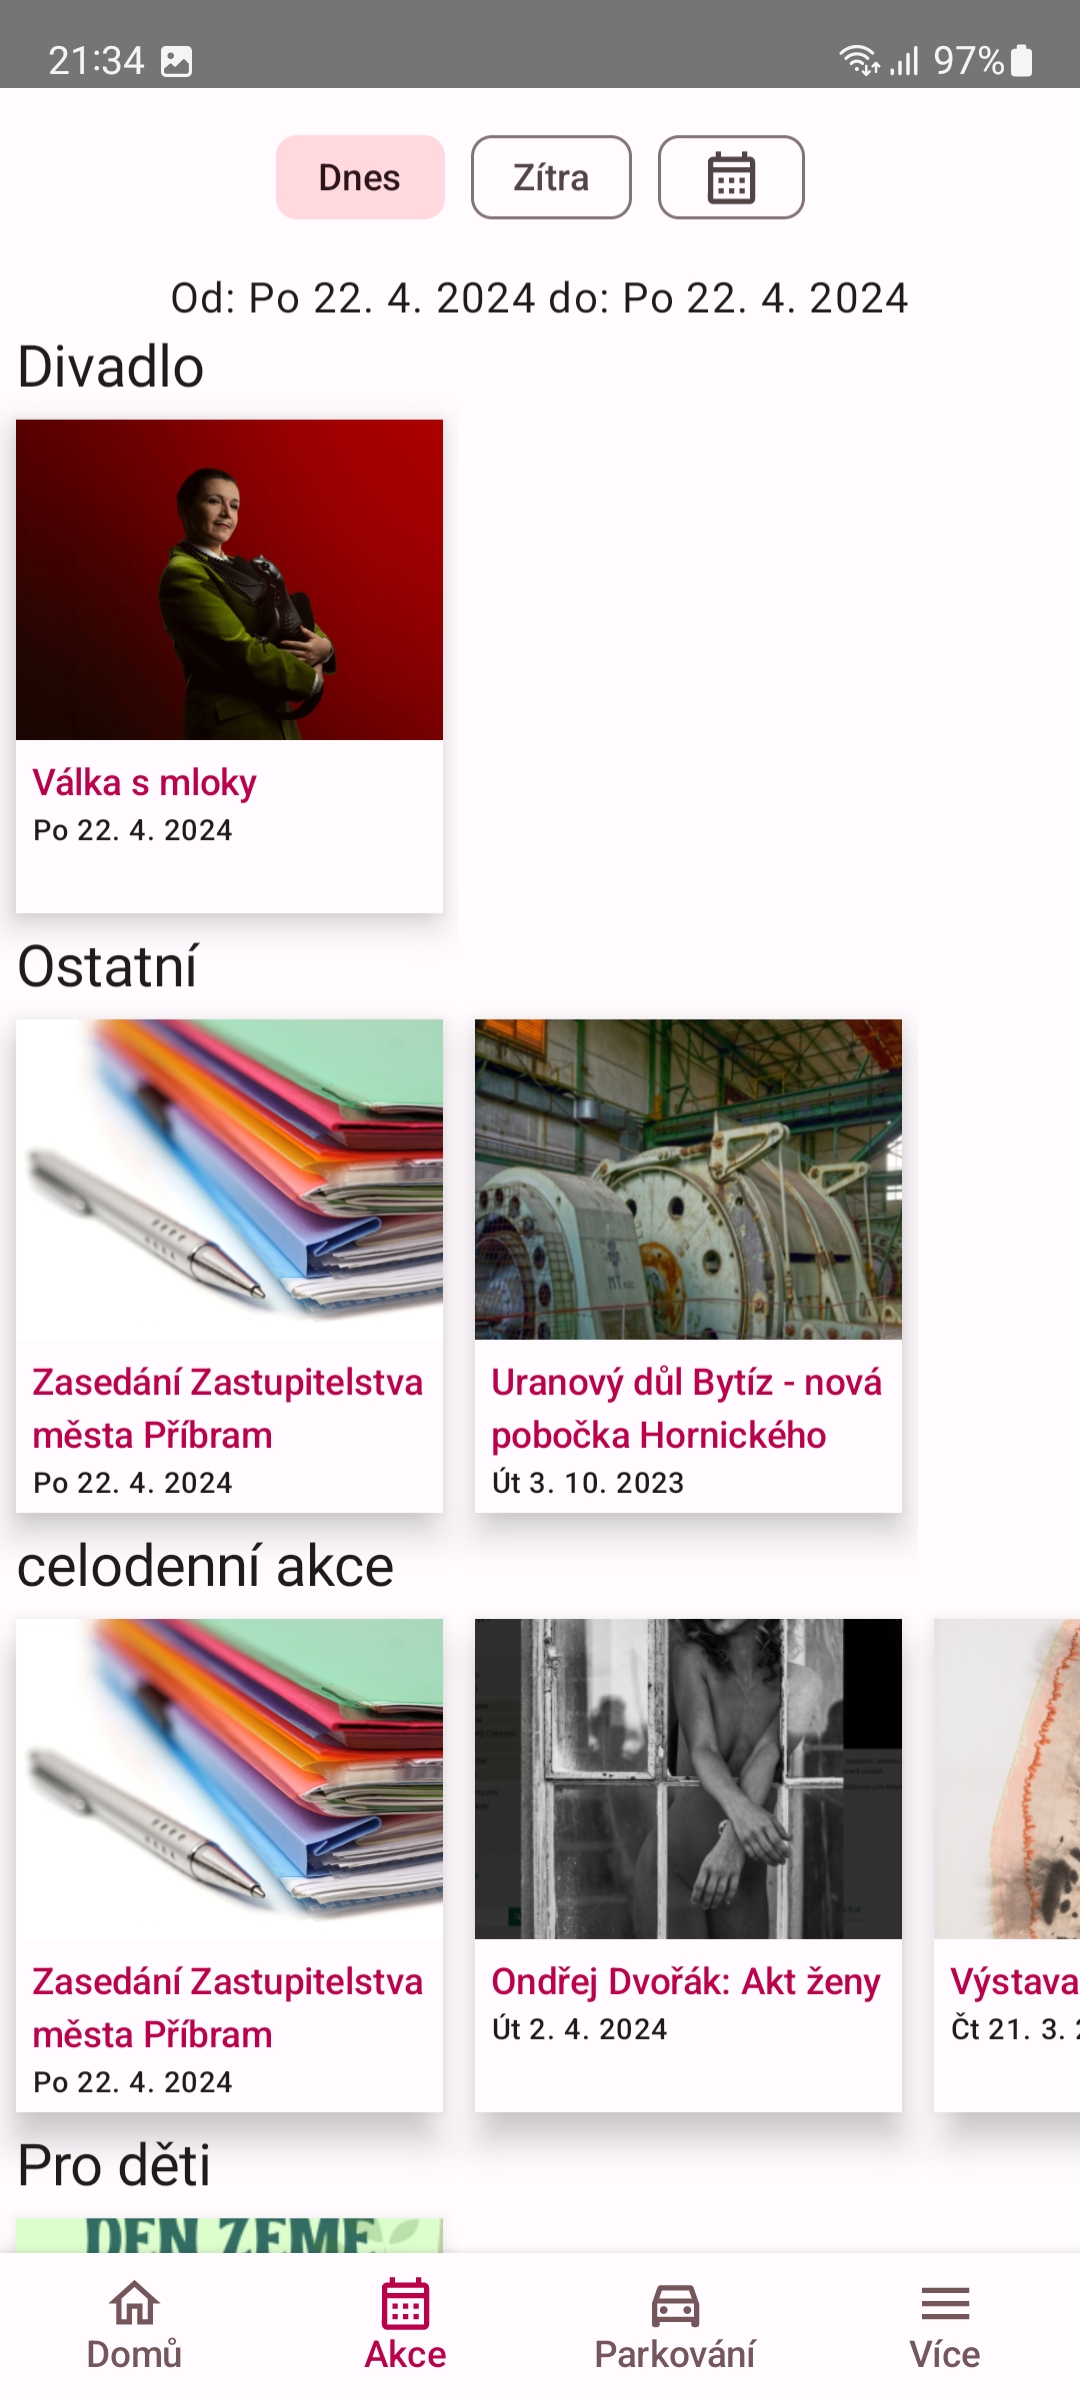
\includegraphics[width=\linewidth]{screens/2.jpg}
    \caption{Obrazovka událostí}
  \endminipage\hfill
  \minipage{0.4\textwidth}
    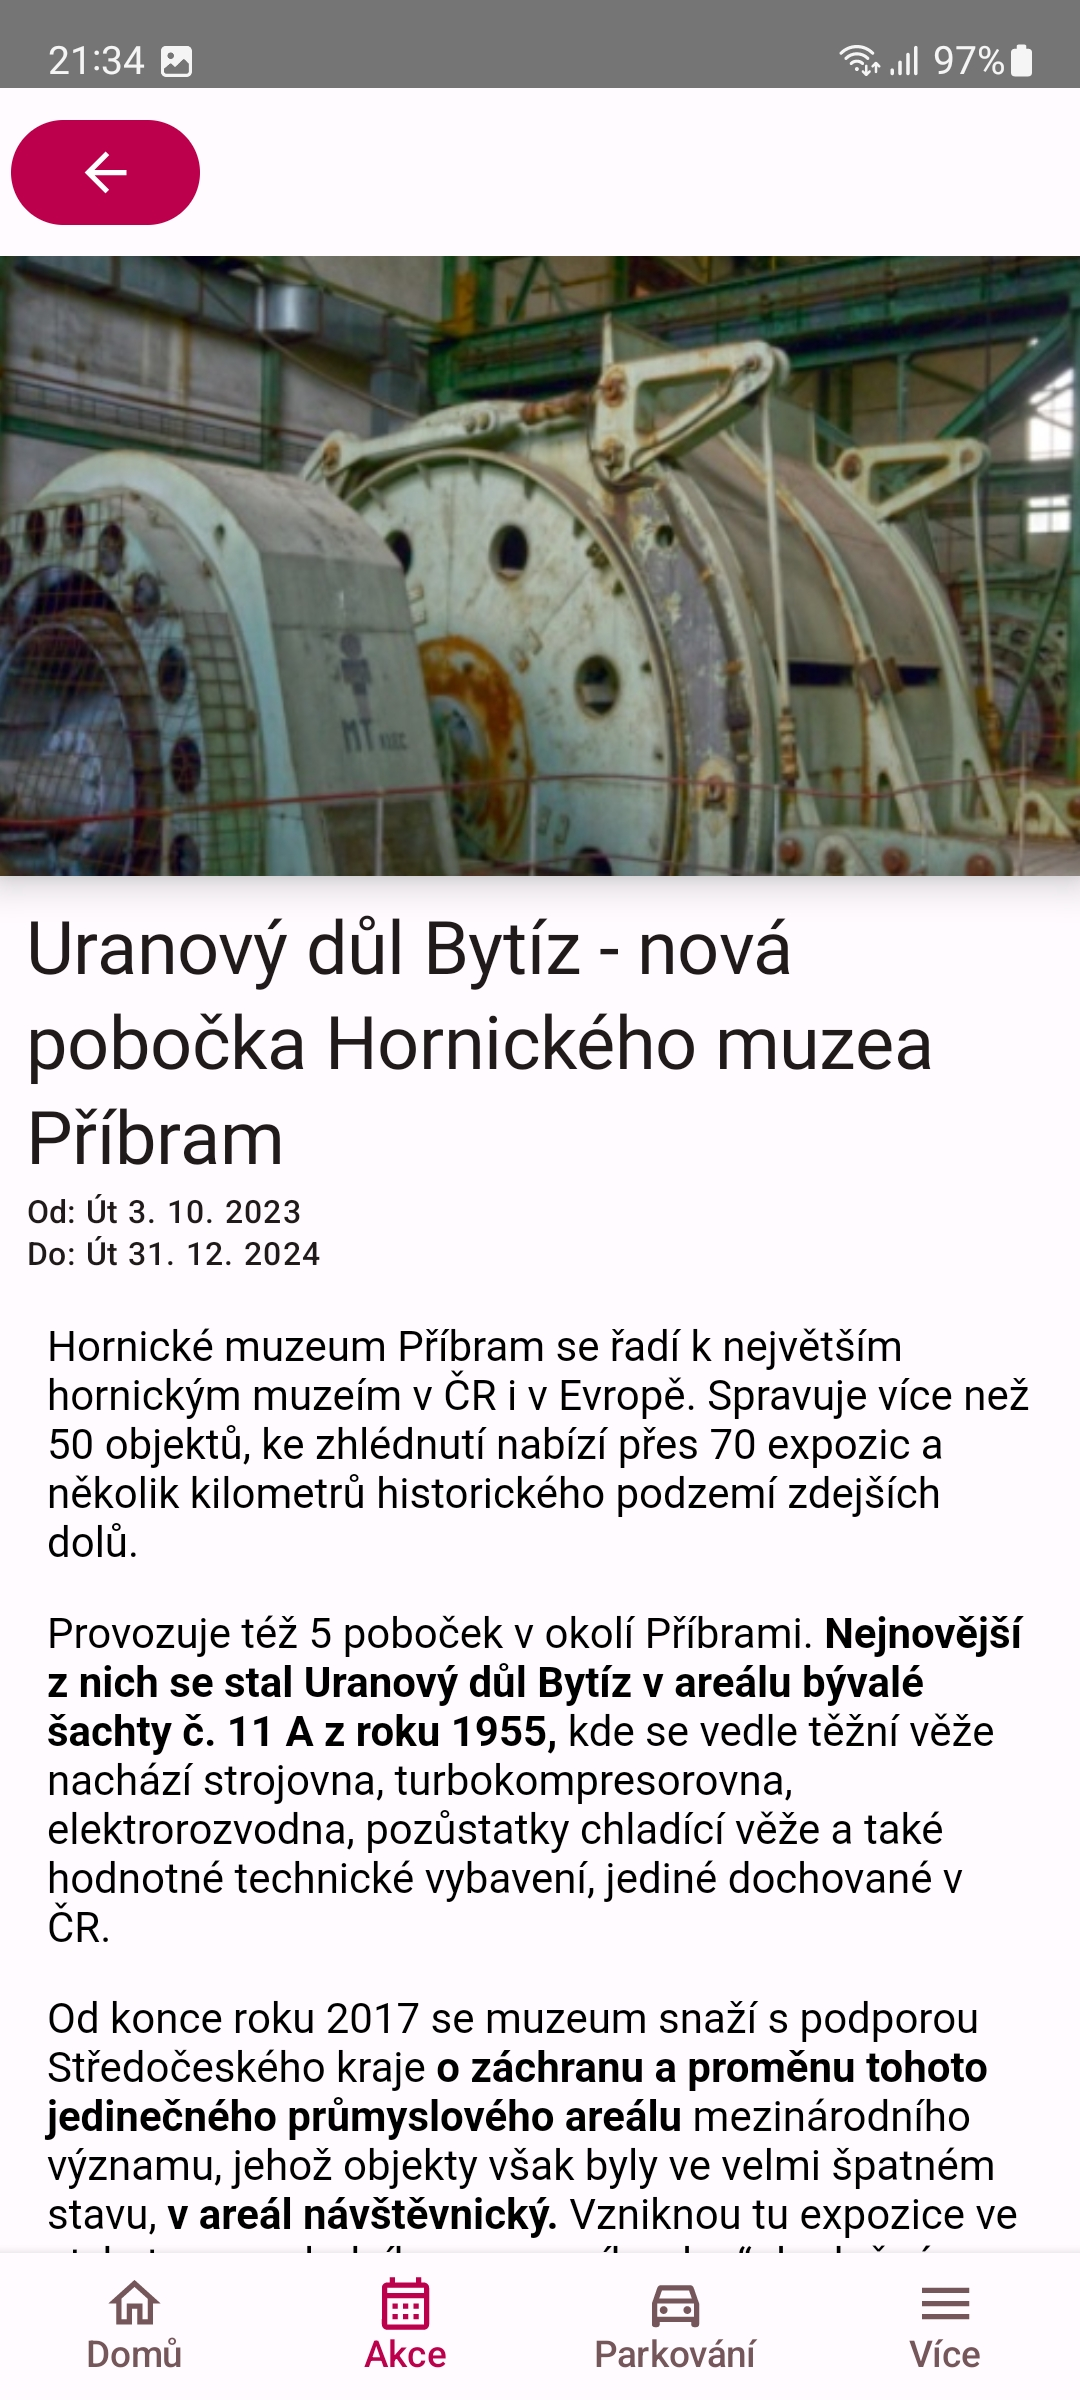
\includegraphics[width=\linewidth]{screens/2a.jpg}
    \caption{Obrazovka událostí}
  \endminipage\hfill
\end{figure}

\begin{figure}[H]
    \minipage{0.4\textwidth}
    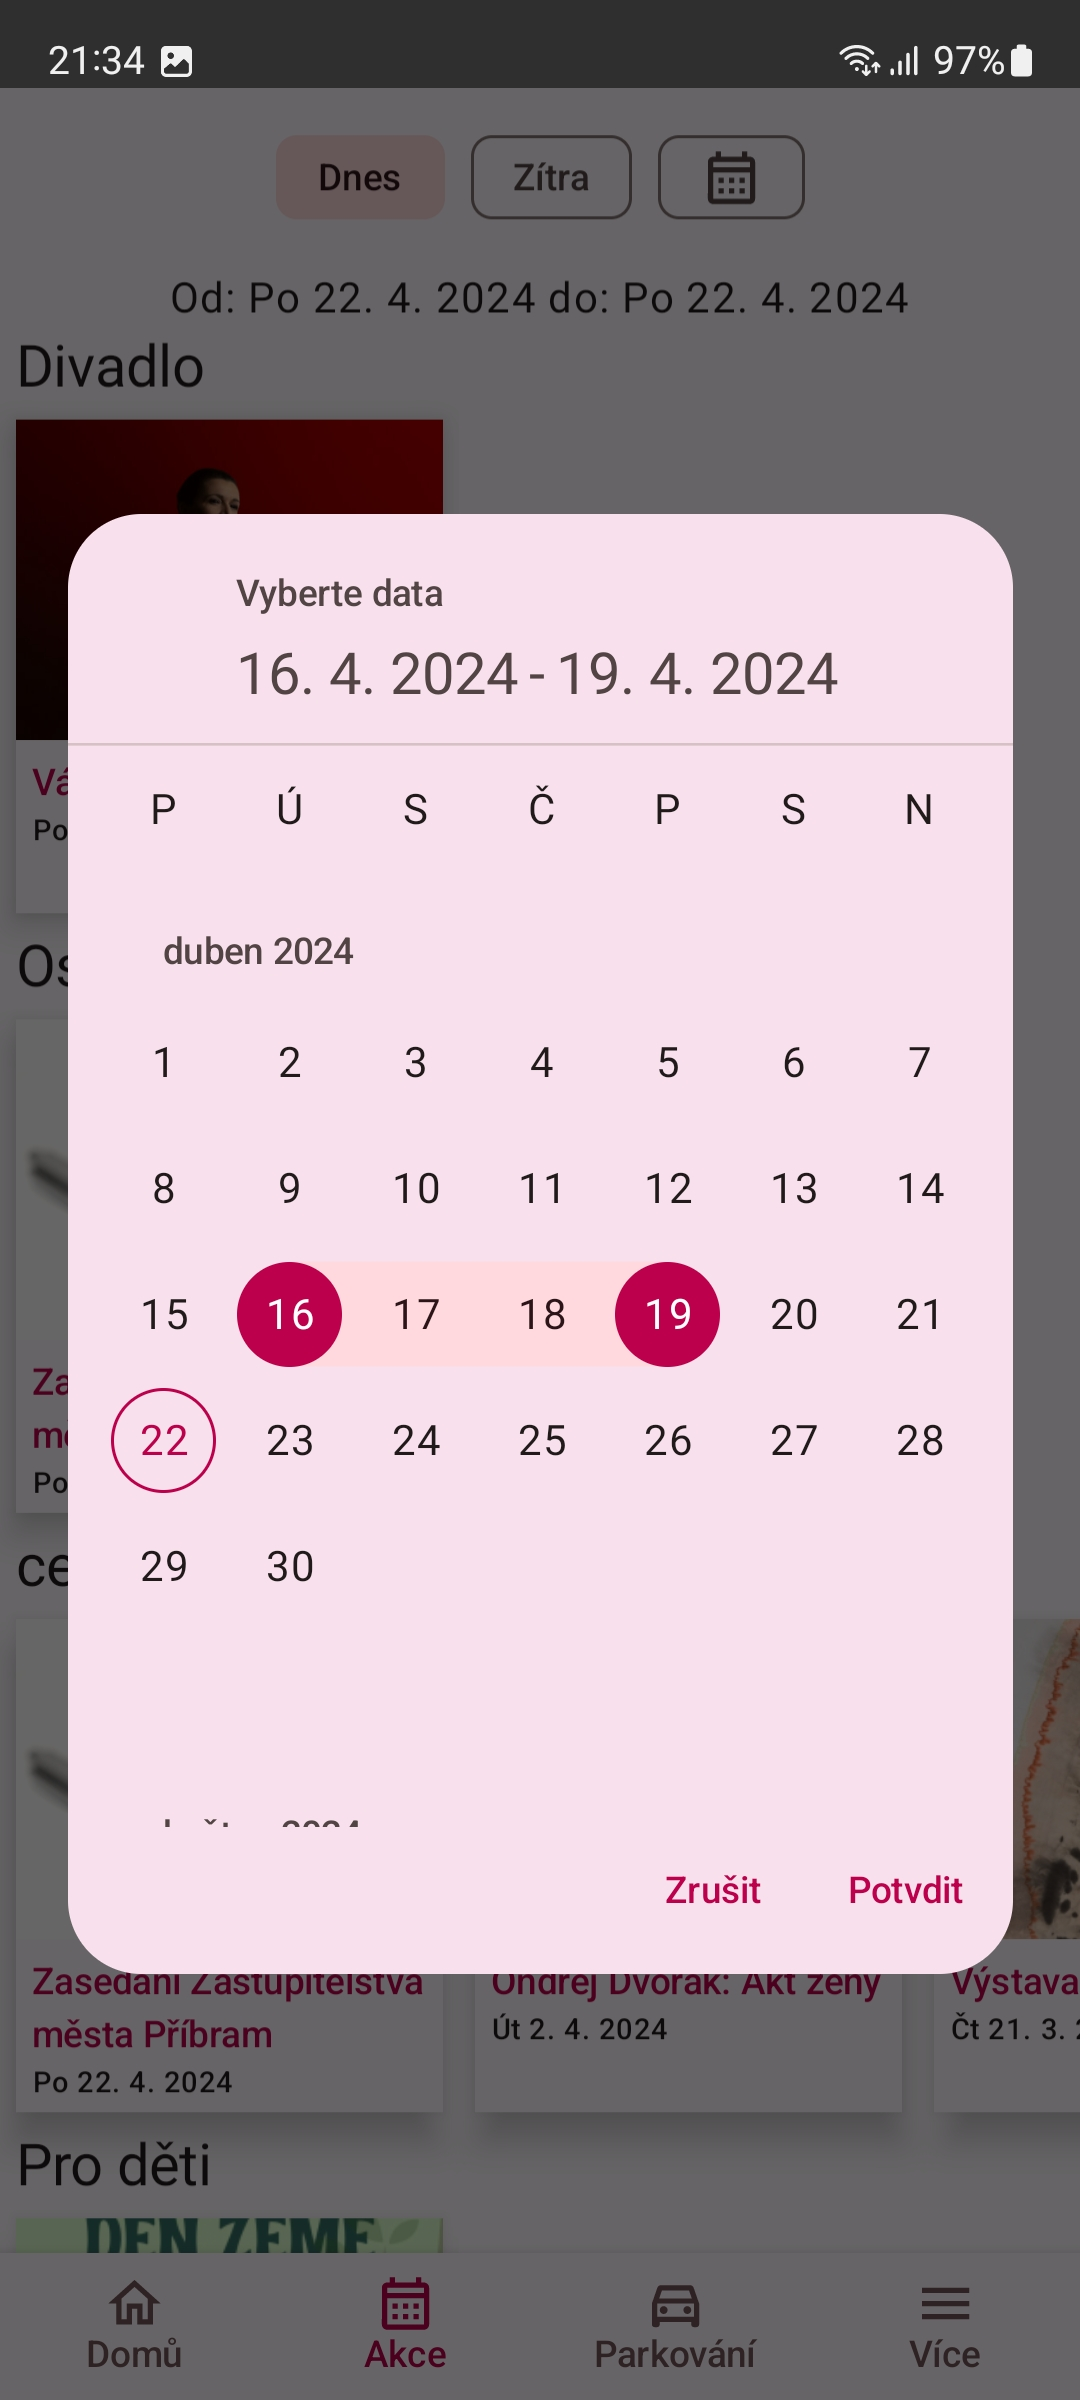
\includegraphics[width=\linewidth]{screens/2b.jpg}
    \caption{Obrazovka událostí}
  \endminipage\hfill
  \minipage{0.4\textwidth}
    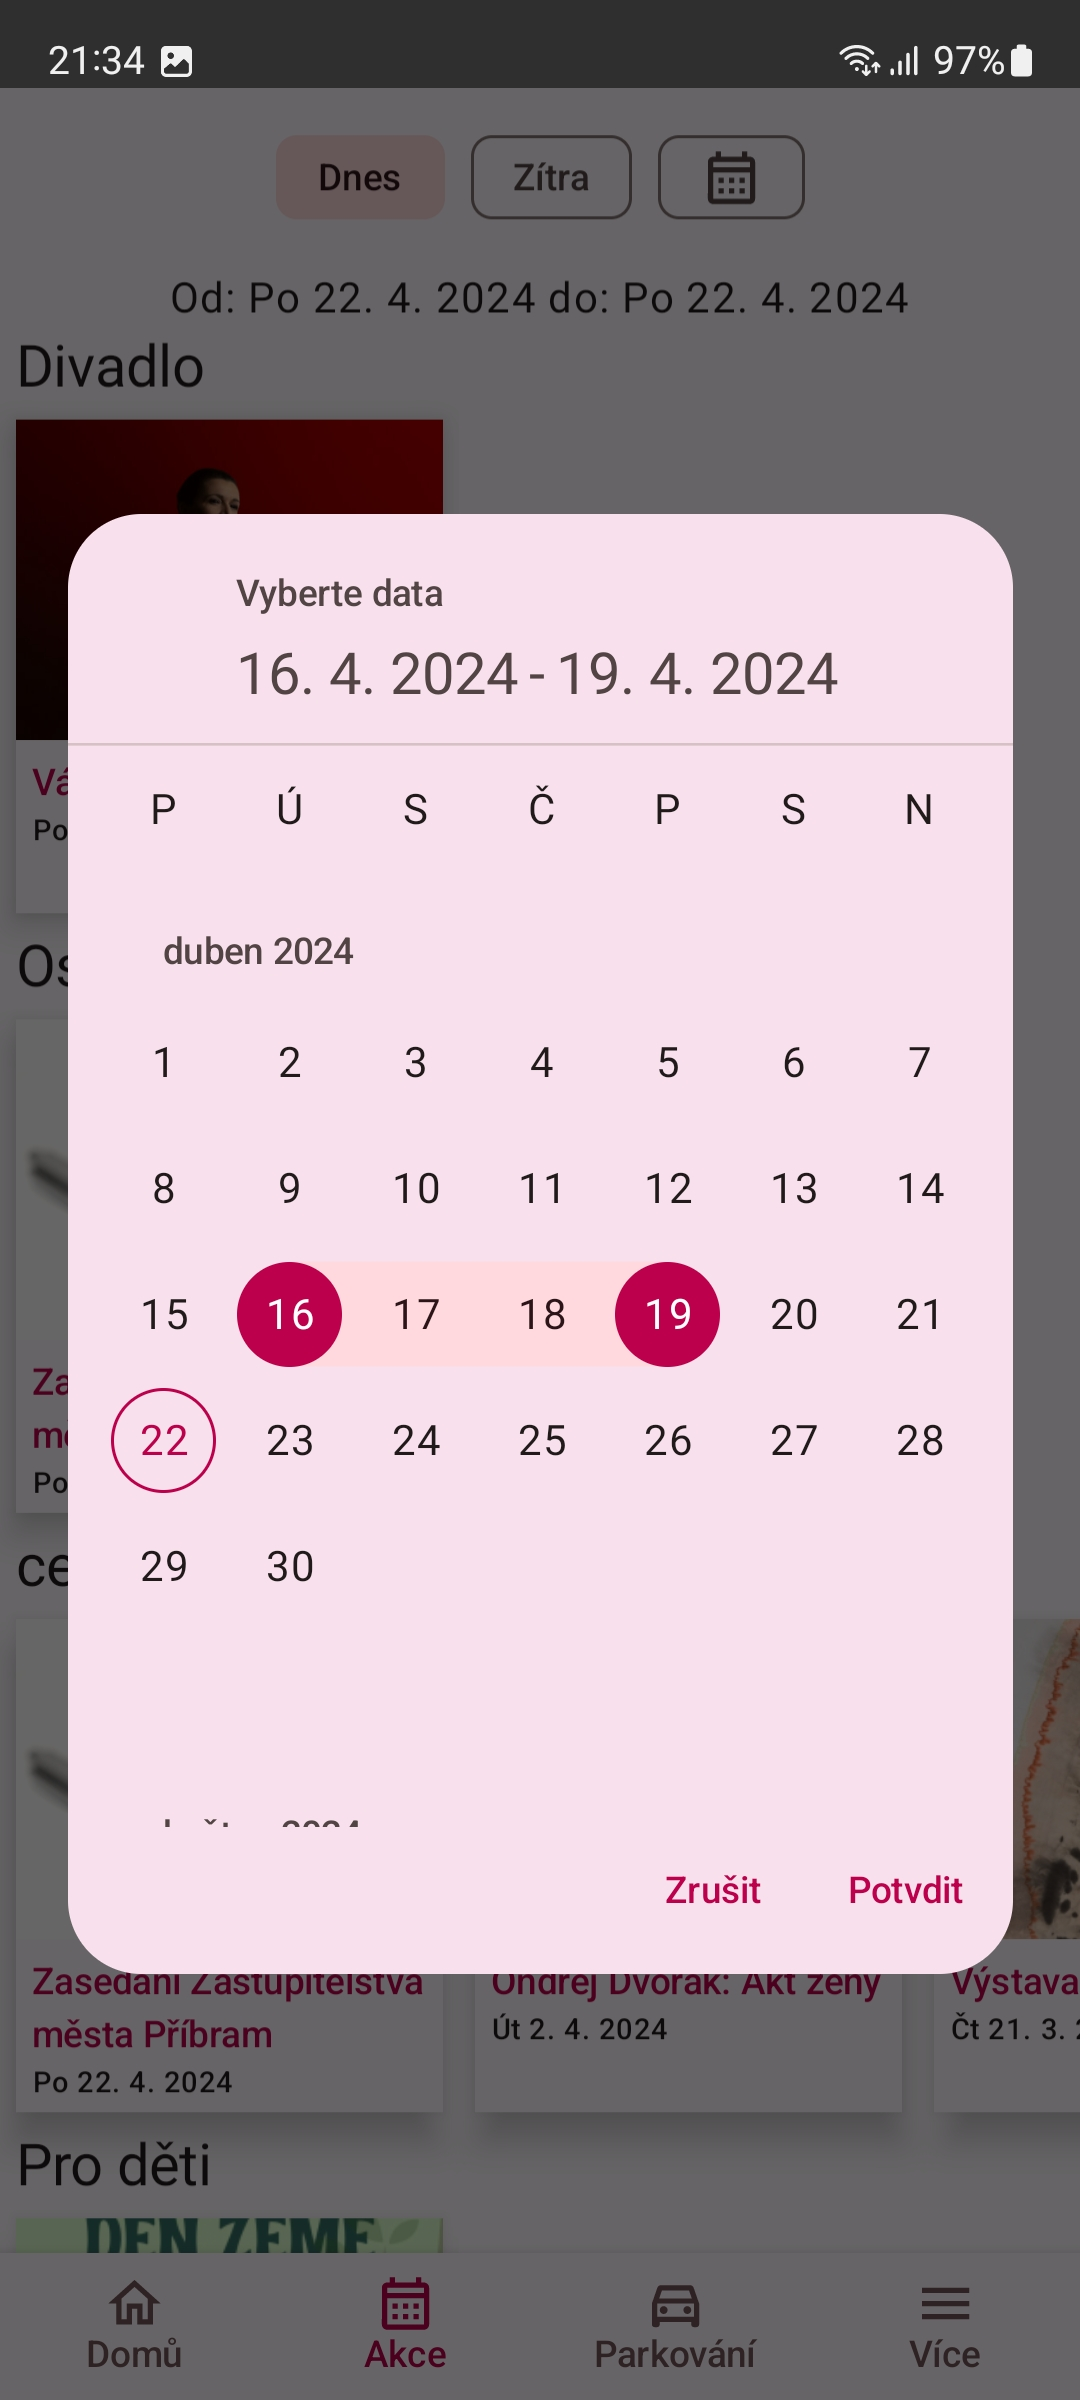
\includegraphics[width=\linewidth]{screens/2b.jpg}
    \caption{Obrazovka událostí}
  \endminipage\hfill
\end{figure}

\begin{figure}[H]
    \minipage{0.4\textwidth}
    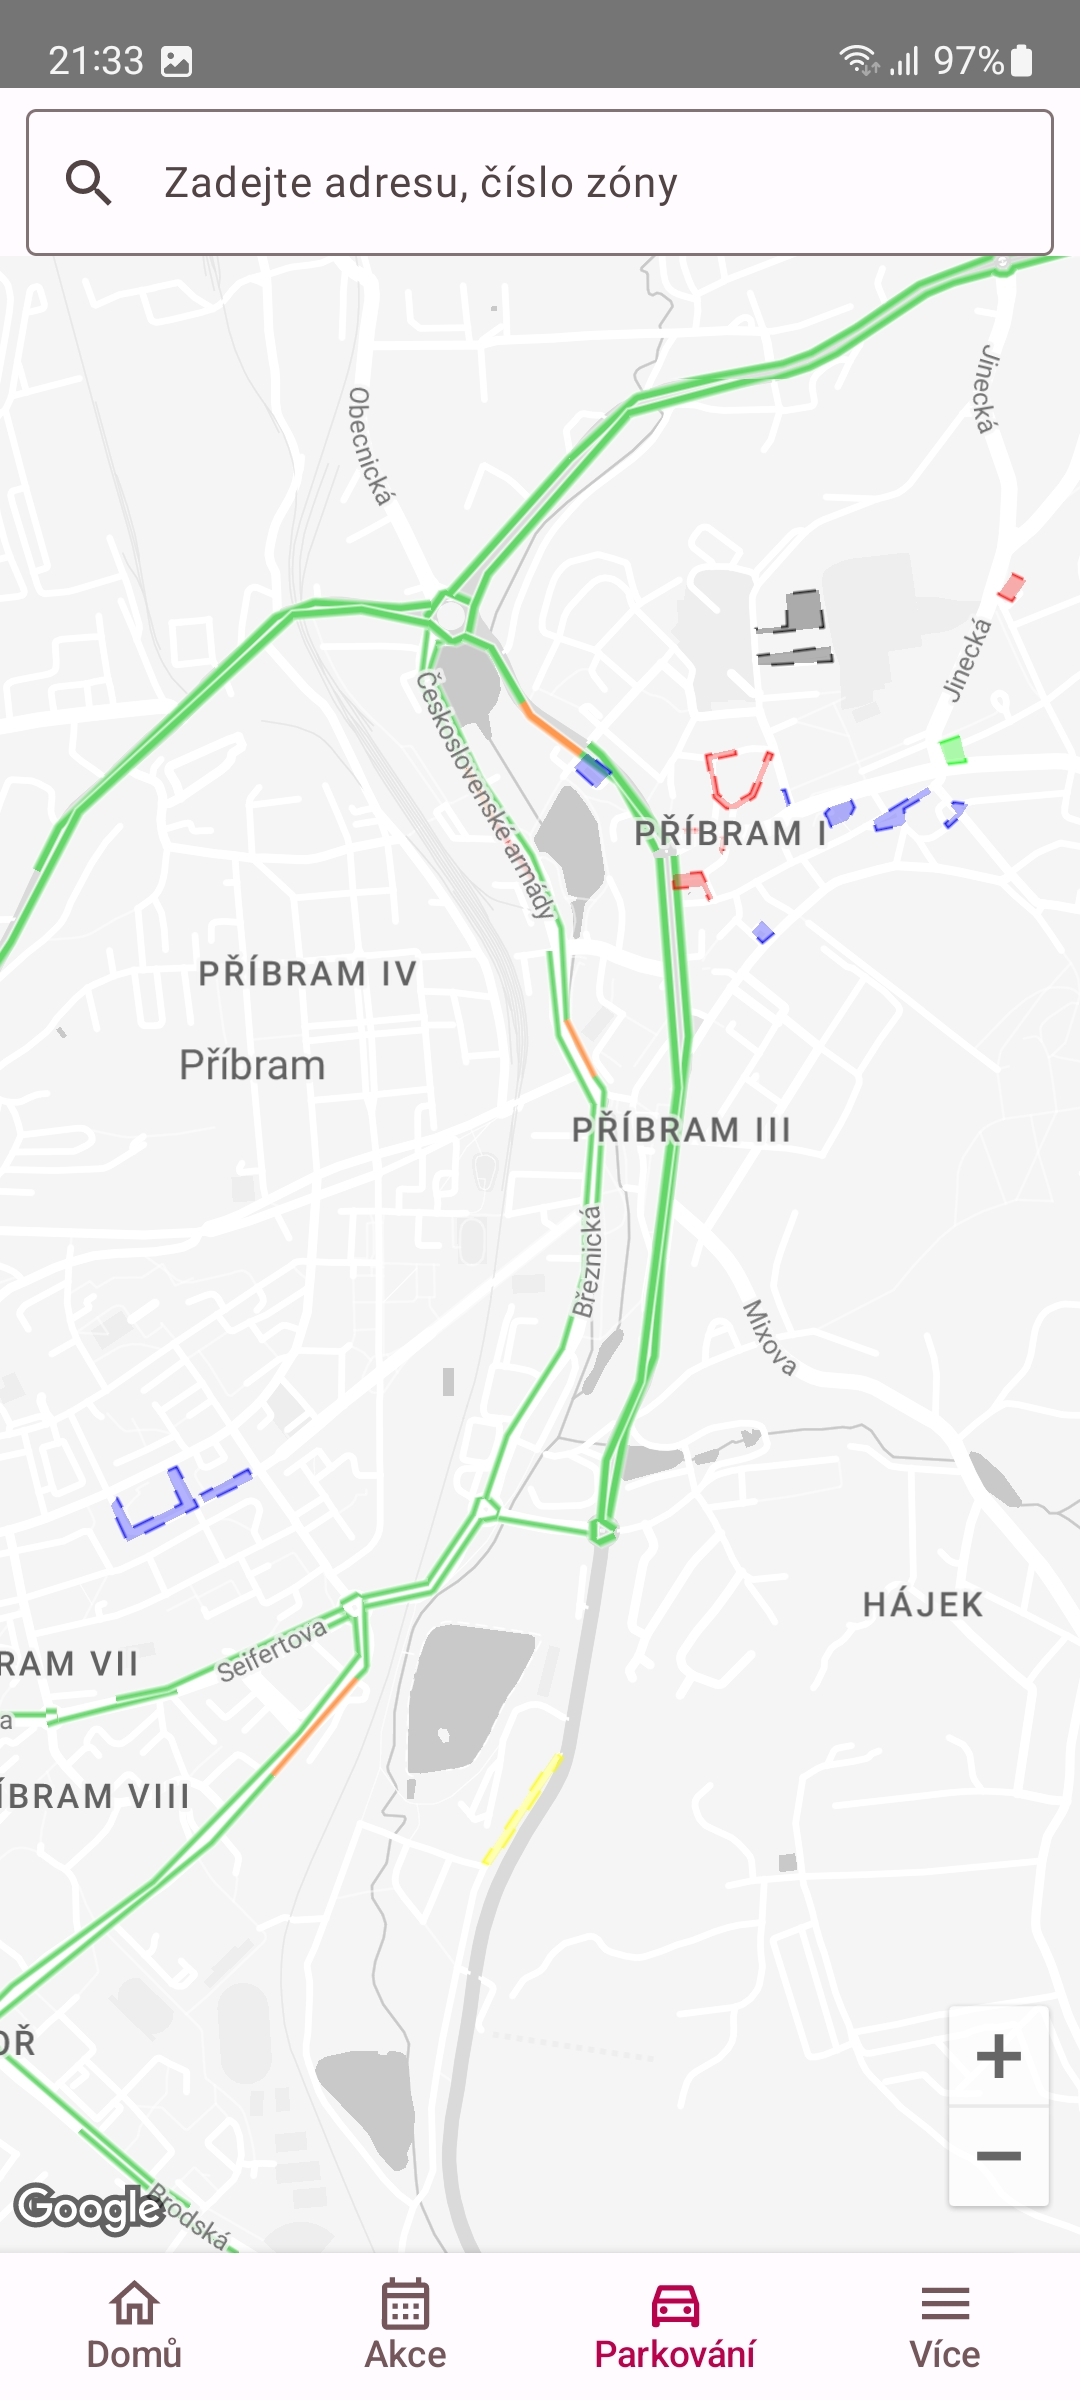
\includegraphics[width=\linewidth]{screens/3.jpg}
    \caption{Obrazovka parkování}
  \endminipage\hfill
  \minipage{0.4\textwidth}
    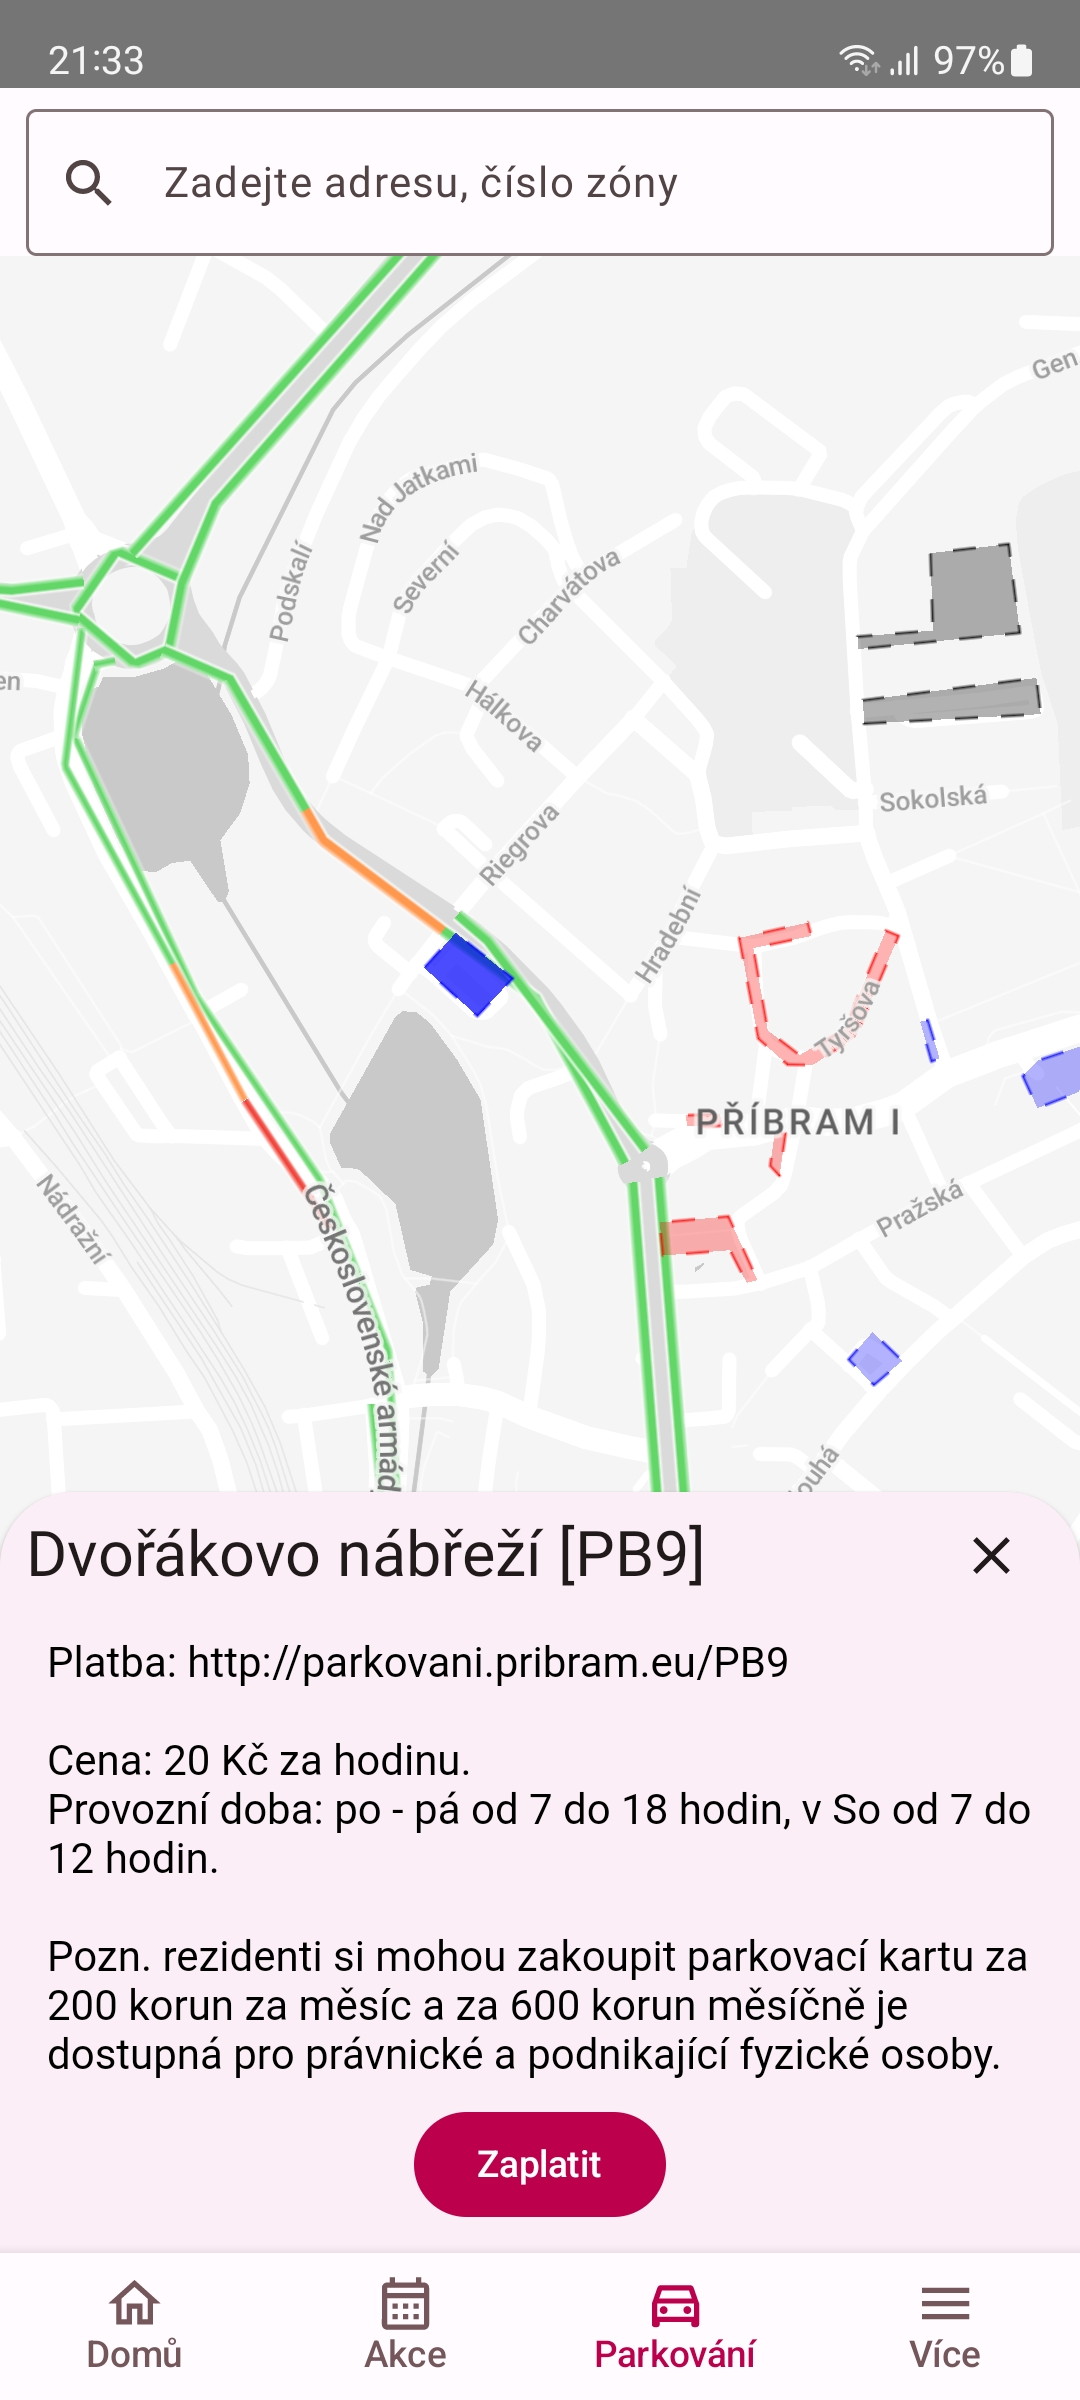
\includegraphics[width=\linewidth]{screens/3b.jpg}
    \caption{Obrazovka parkování}
  \endminipage\hfill
\end{figure}

\begin{figure}[H]
    \minipage{0.4\textwidth}
    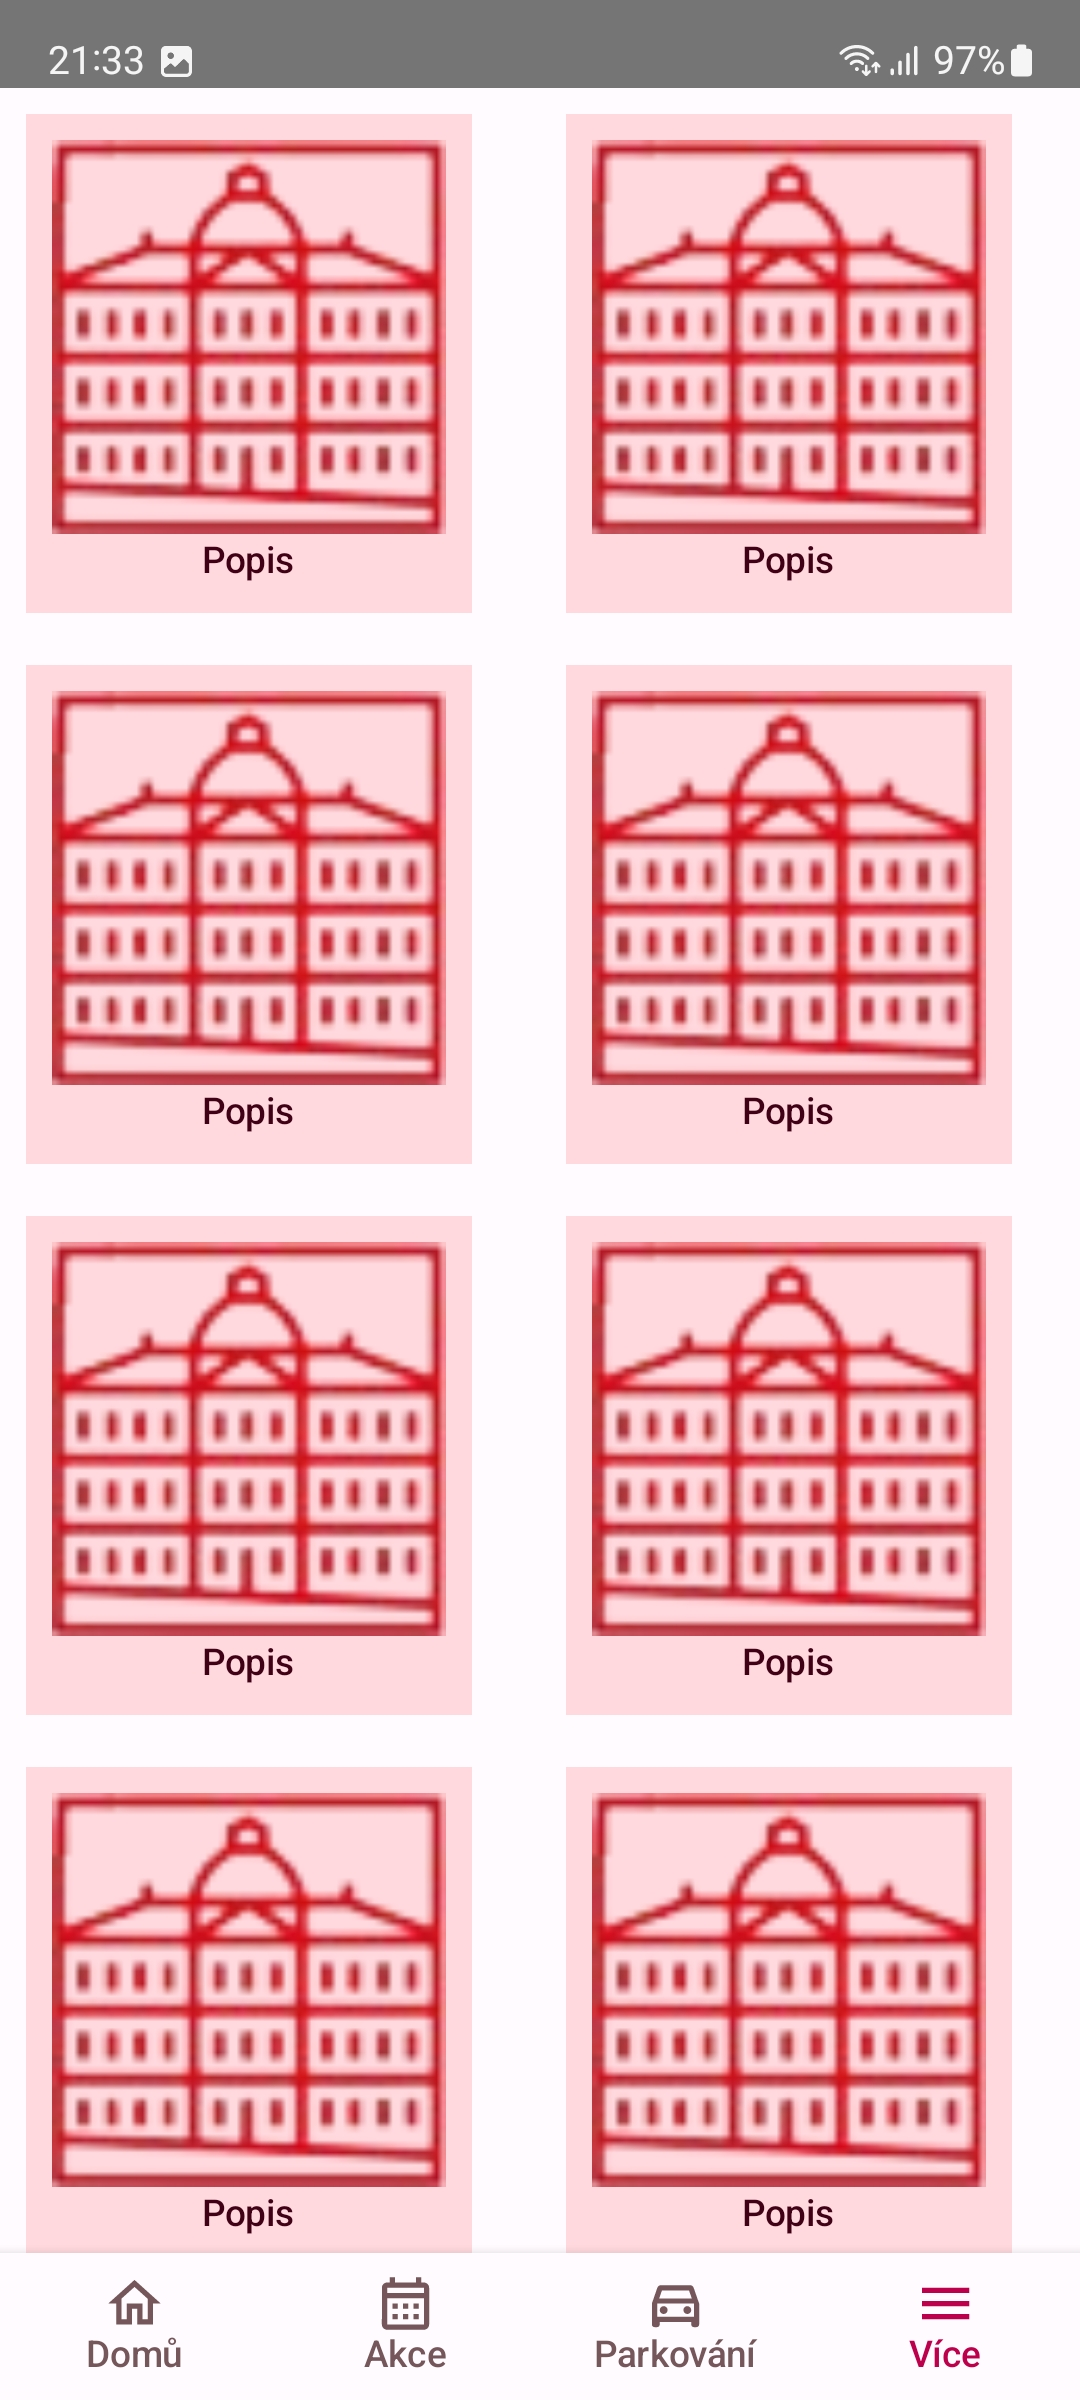
\includegraphics[width=\linewidth]{screens/4.jpg}
    \caption{Obrazovka parkování více}
  \endminipage\hfill
  \minipage{0.4\textwidth}
    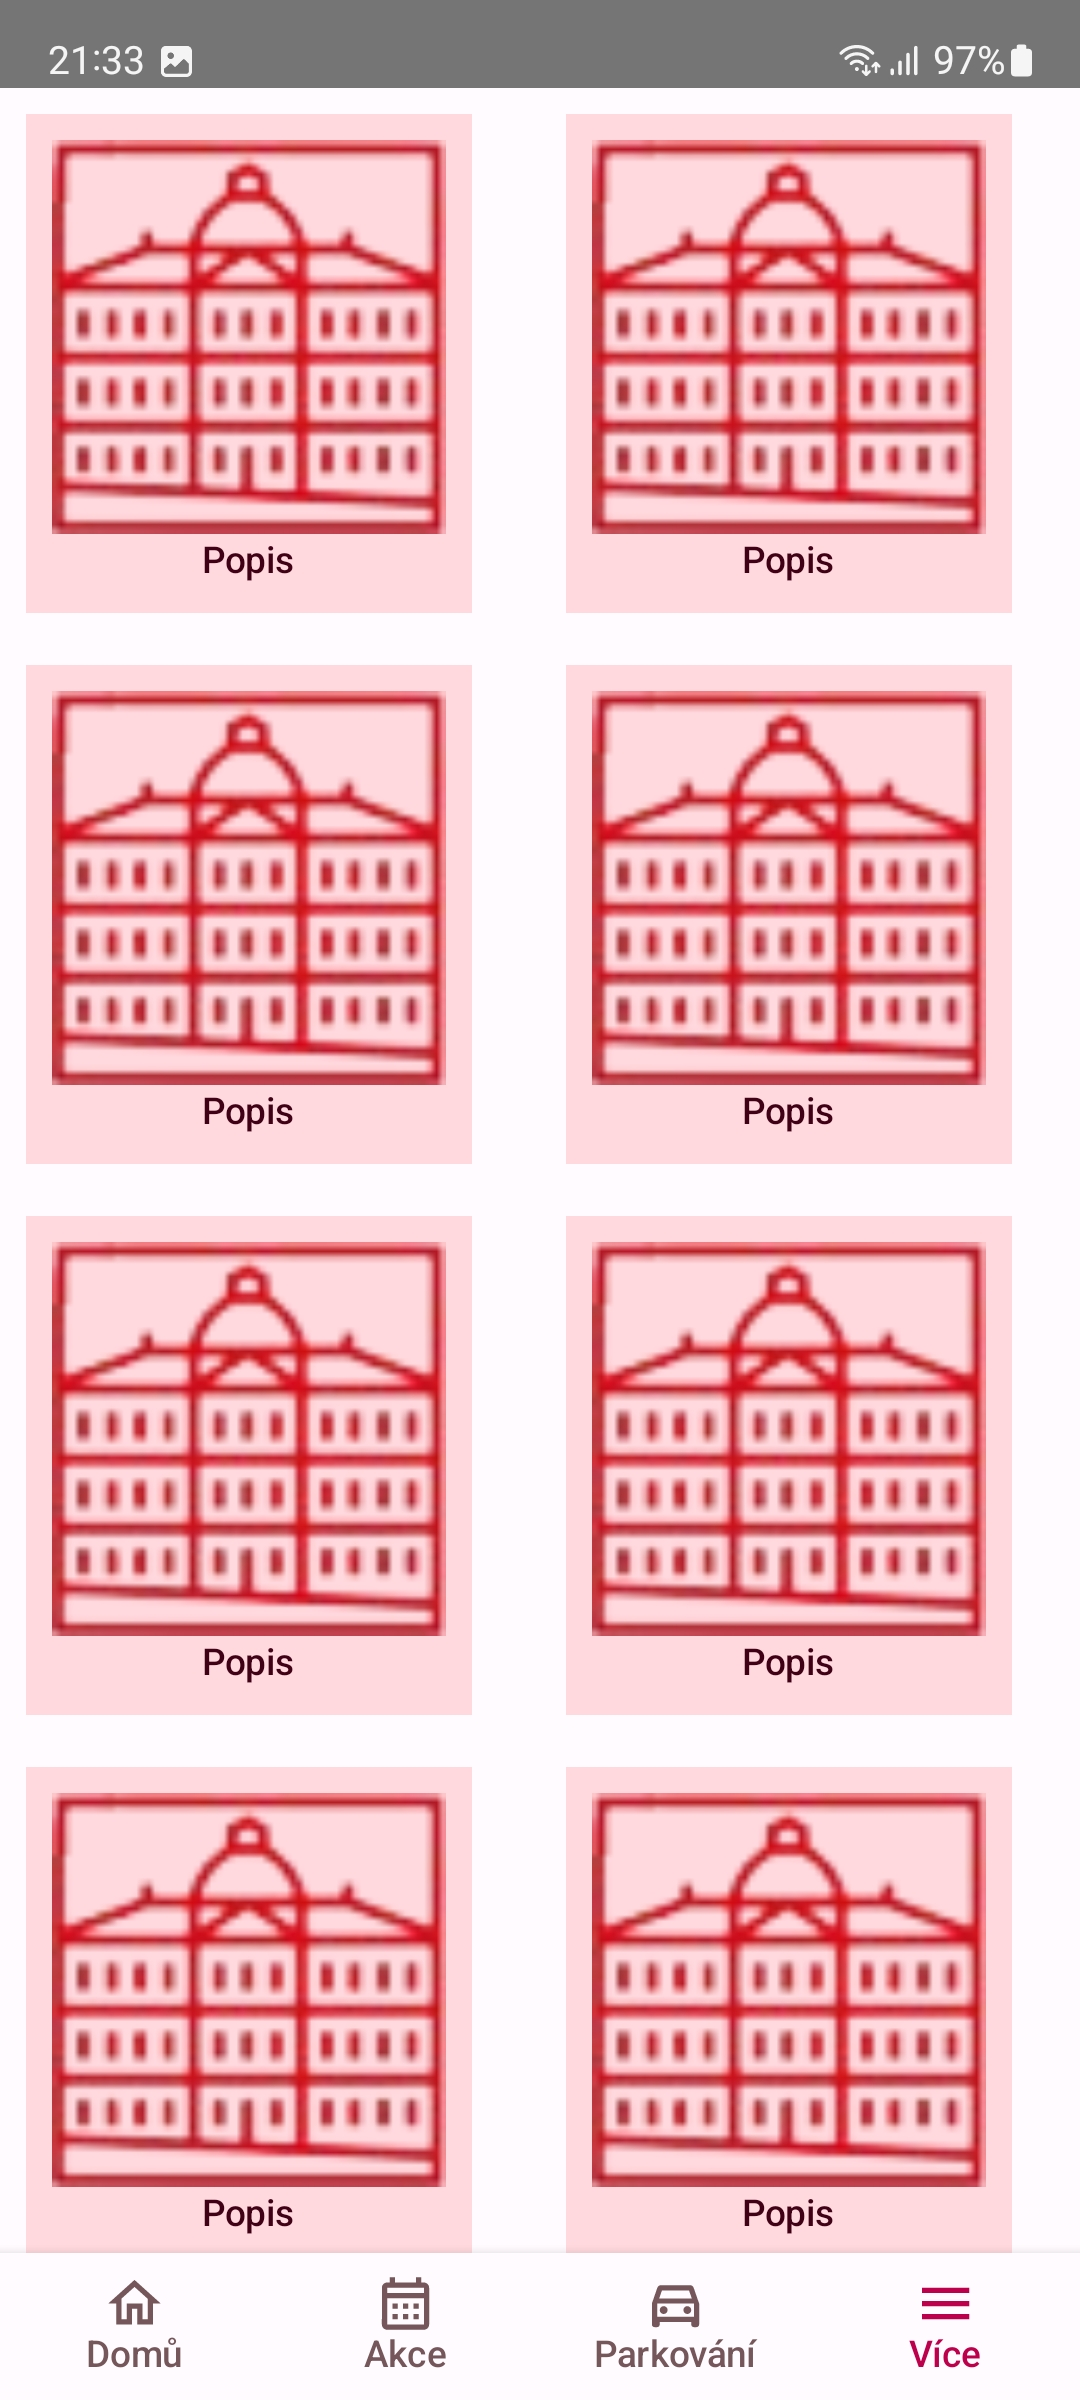
\includegraphics[width=\linewidth]{screens/4.jpg}
    \caption{Obrazovka parkování více}
  \endminipage\hfill
\end{figure}


Sem přijde to, co nepatří do hlavní části.
 % include `appendix.tex' from `text/' subdirectory

\backmatter % do not remove this command

\printbibliography % print out the BibLaTeX-generated bibliography list

\chapter{Obsah příloh}
% Concents of the attachment

	\dirtree{%
		.1 README.md.
		.1 composeMultiplatformProject\DTcomment{kořenovaá složka projektu}.
		.2 composeApp. %\DTcomment{mul}.
		.3 src.
		.4 androdidInstrumentedTestDebug\DTcomment{E2E testy pro platformu Android}.
		.4 androidMain\DTcomment{zdrojové kódy pro platformu Android}.
		.4 commonMain\DTcomment{společné zdrojové kódy}.
		.4 commonTest\DTcomment{společné testy}.
		.4 iosMain \DTcomment{zdrojové kódy pro platformu iOS v jazyce Kotlin}.
		.2 iOS\DTcomment{projektové soubory platformy iOS a kódy v jazyce Swfit}.
		.1 text\DTcomment{text práce}.
		.2 thesis.pdf\DTcomment{text práce ve formátu PDF}.
	}
 % include `medium.tex' from `text/' subdirectory

\end{document}
